\part{Use of ML algorithms with exoplanet spectra and direct imaging maps}
\startcontents[chapters]
\printmyminitoc{}

\chapter{Revisiting the context of the use of ML algorithms for detection and characterization}
In lieu of having a discussion section, we will discuss the results that were produced using the cross correlation algorithm and its consequences for the detection and characterization hypotheses.
Given these consequences, we will then define what the benchmark for the ML algorithms are. 
Finally, we will discuss how these consequences could help the scientific community.
\subsection{The detection hypothesis and the relevant benchmark}
The detection hypothesis states that given the appropriate spectral parameters, it is possible to detect an exoplanet with unlimited sensitivity.
We define sensitivity as the ability to detect faint exoplanets while having $<10^{-4}$ average false positive rate.
We then composed a detection matrix to quantify this sensitivity as a function of the observation parameter $\rm{SNR}$ and the instrumental parameter $R$.
Within this detection matrix we filled the contrast at which the exoplanet was detectable in the spectrum for an $\rm{SNR_{ccf}}\ge6$ for a defined $\rm{SNR}$ and $R$.
We found that $R$ had very little effect on the sensitivity of detection, but beyond a $\rm{SNR}>10^{5}$ the exoplanet at the lowest contrast was detectable at all values of $R$. 
This result has some interesting consequences firstly for the next step whereby it will set the benchmark for the ML algorithms and secondly for the scientific goals of using exoplanet spectra in general.

\paragraph{Setting the benchmark for ML algorithms:\\}
The question that this part of my thesis seeks to answer is whether ML algorithms, with their ability to learn patterns, can learn a generalized pattern corresponding the features of exoplanet spectrum to identify those spectra which contain them.
We define this problem to be complicated by three broad parameters, $C,R \& \rm{SNR}$.
The detection matrix allows us to establish where in the parameter space are traditional algorithms most sensitive to the exoplanet. 
We have now established that to have the highest sensitivity, the cross correlation algorithm requires a minimum $\rm{SNR} =10^{5}$.
This then implies that there definitely is enough planetary features which could be matched with a template.
The detection matrix also justifies that $R$ has very minimal to no impact on  detection sensitivity.
Therefore, the first benchmark goal for ML algorithms would be two fold,
\begin{enumerate}
    \item within the parameter space that the cross correlation detection algorithm achieves its highest sensitivity, the ML algorithm also needs to perform as well and this will be quantified using confusion matrices to begin with and 
    \item if ML algorithms achieve a mean false positive rate $<10^{-4}$ and true positive rate $>0.5$ in this parameter space, they will be used to construct a similar detection matrix.
\end{enumerate}
This step would validate that ML algorithms are indeed a reasonable replacement for the cross correlation algorithm. This means that ML algorithms through this methodology can be used to estimate the sensitivity of datasets.
Finally, for ML algorithms to be considered better than cross correlation based algorithms it needs to satisfy the following conditions, in addition to the above,
\begin{enumerate}
    \item they need to be more sensitive to fainter companions, with the same false positive rate, at lower $\rm{SNR}$ and
    \item to be just as flexible with increasing $R$ with the same sensitivity.
\end{enumerate}
\paragraph{Consequence for the scientific goals of spectral data processing to detect exoplanets:\\}
The detection matrix allows us to estimate the parameter space that is ideal for detection sensitivity to be maximized.
It also allows us insight into certain parameters that limit the detection sensitivity.
One of the key goals of scientific data collection and processing is to identify the values within parameter space that allows us to achieve the scientific goals.
The detection matrix aims to be the basis to establish these values for specific scientific cases.
The scientific case that we make at this point is the detectability of warm Jupiters using spectra at different $\rm{SNR}$ and $R$.
More specifically, we aim to define at what contrasts are these warm Jupiters detectable.
In the case of warm Jupiters, it is clear the $\rm{SNR}$ is the most important parameter that limits the sensitivity of detection.
An interesting observation is that this sensitivity does not change with increasing $R$ where the $\rm{SNR_{\lambda}}$ decreases for a fixed $\rm{SNR}$.
The detection sensitivity is thus directly related to the overall $\rm{SNR}$ than to the $\rm{SNR}_\lambda$ for each wavelength bin.
Therefore, using this matrix it is clear that for $\rm{SNR}=10^{4}- 10^{5}$, which is the mean $\rm{SNR}$ that is achieved for an observation such as \textcolor{blue}{[Refer to observations in Part II HD142527b]} we will be able to detect a warm Jupiter at a $C\approx 10^{-4}$.

Another interesting consequence, is the rate at which sensitivity improves in the detection matrix.
In Fig~\ref{fig:parspace-1} it was clear that there is a linear relationship between the $\rm{SNR}$ and $\rm{SNR_{ccf}}$ particularly beyond $\rm{SNR_{ccf}}\ge 5$.
This means that beyond this value an increase in $\rm{SNR}$ produces a an increase on $\rm{SNR_{ccf}}$ in the detection matrix as it is composed of only contrasts where the $\rm{SNR}_{ccf}>6$.
Thus for an increase in $\rm{SNR}$ we should logically see a uniform increase in the detected $C$. However, what we observe is that this increase is not uniform, whereas it increases quite rapidly for lower contrasts $C<10^{-4}$ but increases much slower for higher contrasts.
This is a very interesting behaviour which seems to indicate that for this sort of data detections beyond $10^{-4}$ may be difficult to pass.
We will see this progress in more detail in \textcolor{blue}{[Refer Part II Chapter results]}.

Finally, we see that for increase in $R$ there is little to no impact on detection. 
This is particularly interesting, because we would expect that for a constant $\rm{SNR}$ an increase in $R$ will produce a drop in $\rm{SNR_{\lambda}}$. 
This means each of the wavlength bins have fewer signal photons and therefore the cross correlation strength should reach $\rm{SNR}_{ccf}=6$ only when more overall photons are available (i.e at higher $\rm{SNR}$. 
But it appears that overall $\rm{SNR}$ (which is constant along a row) is the only aspect that influences detection and not $\rm{SNR_{\lambda}}$.
We posit that this is the case because of the large number of wavelength bins available, the mean $\rm{SNR}$ is a bigger factor than individual photons in individual bins.
Thus the advantage of higher resolution can be seen for this problem with not losing sensitivity to detection.
This might have been a very good case for higher resoluion instruments if the characterization showed improved results with resolution.
\subsection{The characterization and its relevant benchmark}
\label{sec:removal of stellar}
Characterization, in this thesis, is defined as being able to constrain the $\rm{T_{eff}}$ and $\log(\rm{g})$ of an exoplanet with consistent error bars.
Our characterization hypothesis states that we should be able to characterize any spectrum where an exoplanet exists.
The word exists is precisely quantified by the detection algorithm as having a $\rm{SNR_{ccf}}\ge 5$.
This is evidenced when we use the characterization matrix on spectra at fixed $R,C$ and varying $\rm{SNR}$.
We notice that the $\rm{T_{eff}}$ constraints become consistent after after an $\rm{SNR_{ccf}}\approx 3.5$.
It is, therefore, clear that the quantification of the characterization parameters are heavily influenced by the ability to detect exoplanet spectra. 

We designed a characterization matrix with two things in mind,
\begin{enumerate}
\item to constrain the mean $\rm{T_{eff}}$ and $\rm{\log(g)}$ of a spectrum with an exoplanet along with the independent uncertainties of both these quantities and also,
\item to ensure that we are able to do this for all spectra where a exoplanet spectrum can be detected.
\end{enumerate}
The goal of this matrix is not to quantify the evolution of the error bars or the mean of the $\rm{T_{eff}}$ and $\rm{\log(g)}$ with spectral parameters such as $\rm{SNR}$ and $R$ unlike the detection matrix.
However there are still some interesting points to note and these points will define the characterization goals for ML algorithms.
This involves three broad ideas,
\begin{enumerate}
    \item the evolution of the characterization accuracy,
    \item the impact of the stellar subtraction on characterization accuracy and
    \item the intimate relationship between detection and characterization.
\end{enumerate}
\paragraph{Evolution of the characterization accuracy with the parameter space:\\}
When comparing the error bars over a parameter space we will use the detection matrix in Fig~\ref{fig:detmat} for two purposes,
\begin{enumerate}
    \item to make the link between \textit{detectability} and accurate characterization of the exoplanet spectrum
    \item and secondly to demonstrate the handy of the detection matrix when describing the evolution of science goals (in this case detection and characterization) with the parameter space.
\end{enumerate}
When we look at the evolution of both $\mu_x$ and $\sigma_x$ in the characterization matrix in Fig~\ref{fig:nondet_char} to Fig~\ref{fig:charmap-det} the first point is the evolution of the $\mu_x$ i.e the mean $\rm{T_{eff}}$ and $\rm{\log(g)}$ does not got any closer to the template $\rm{T_{eff}}=1500$K as we move along the rows in the detection matrix.
This property is also true for the $\log(g)$. 
This is a marked diversion from the behaviour of the cross correlation algorithm when used as a detector.
While moving along rows we detect fainter exoplanets, it does not seem to translate that this implies the template is closer (i.e accurate mean) to the one that was inserted.
As we move further along the rows and we increase the $\rm{SNR}$ to more than double, we still see little to no effect on the detection accuracy and it appears that even now there is no way to have a perfect characterization.
This once again marks a departure with detectability where as we move to unphysically high $\rm{SNR}$ values in the top rows we get an almost uniformly perfect sensitivity to detection.

Following this line of thought, the evolution in the $\sigma_{\rm{T_{eff}}}$ and $\sigma_{\rm{\log(g)}}$ is also unsurprising.
However, what is surprising is the fact that error bars remain for as large as two grid points for the $\rm{T_{efF}}$ and slightly more than one grid point for $\log(g)$.
The question, therefore, is what is producing this large error bar. 
The fact that even with higher $R$ this problem is not alleviated shows that intrinsically there is an uncertainty produced by a single quantity left untouched so far i.e $C$.
When we reproduce the same plots for $C=10^{-1}$ which is not only physical but does not have any other detection analog, we see that we get near perfect characterization.
\begin{figure}[!ht]
    \centering
    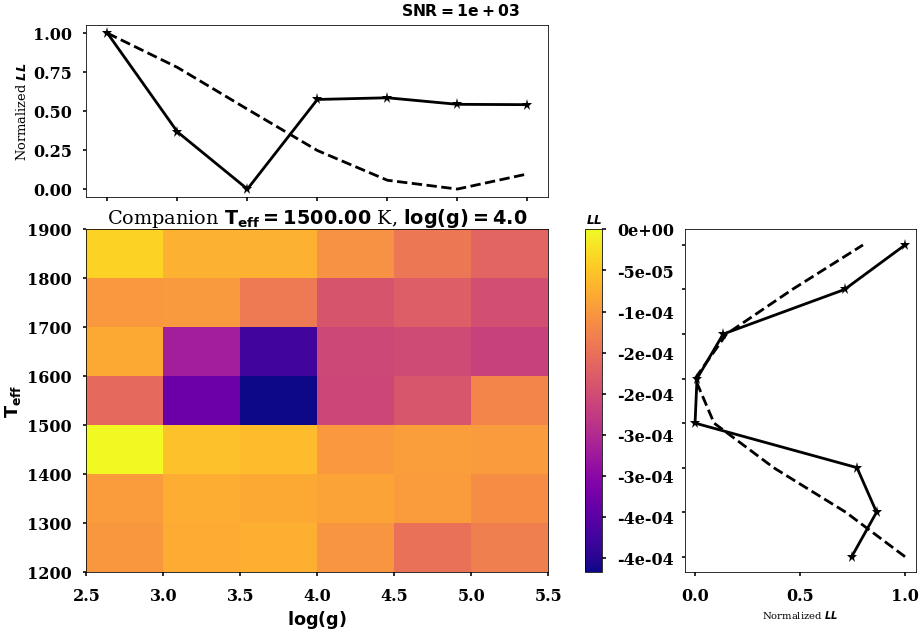
\includegraphics[scale=0.5]{images/Chapter3/char_fits_0.png}
    \caption{Caption}
    \label{fig:perfectchar}
\end{figure}
An example is shown if Fig~\ref{fig:perfectchar}.
We also show the fits to convince ourselves that indeed this fit is an inverse Gaussian fit and the contrast is the parameter the produces a more accurate $\mu_{\rm{T_{eff}}}$.
But even though the mean $\rm{T_{eff}}$ is accurately retrieved there is a fairly large error in the $\log(\rm{g})$ characterization.
But from this map it is fairly clear what the reason for the inaccurate $\rm{T_{eff}}$ characterization is.
If indeed the characterization accuracy and thereby its error bars are constrained by the presence of stellar contaminants, would there be a better accuracy when the star is switched off?
\textcolor{red}{Talk about the ML characterization goal}
\paragraph{Effect of perfect removal of stellar signal from the data:\\}
While this thesis relies on limited pre-processing and is indeed tuned to removing any stellar features from the data, no pre-processing is perfect and leaves some residual stellar contamination in the data.
An easy way to test this is to `switch off' the star and this is fairly easy to do with synthetic data by setting $C=1$ in Eq~\ref{eq:insertion}.
This would be the case where the stellar signal is perfectly subtracted. 
Note that the data still contains observation noise and contains the intrinsic randomness of that noise.
We computed different characterization matrices for such spectra for different $\rm{SNR}$ and $R$ (note that $C=1$ is now a constant).
\begin{figure}[!ht]
    \centering
    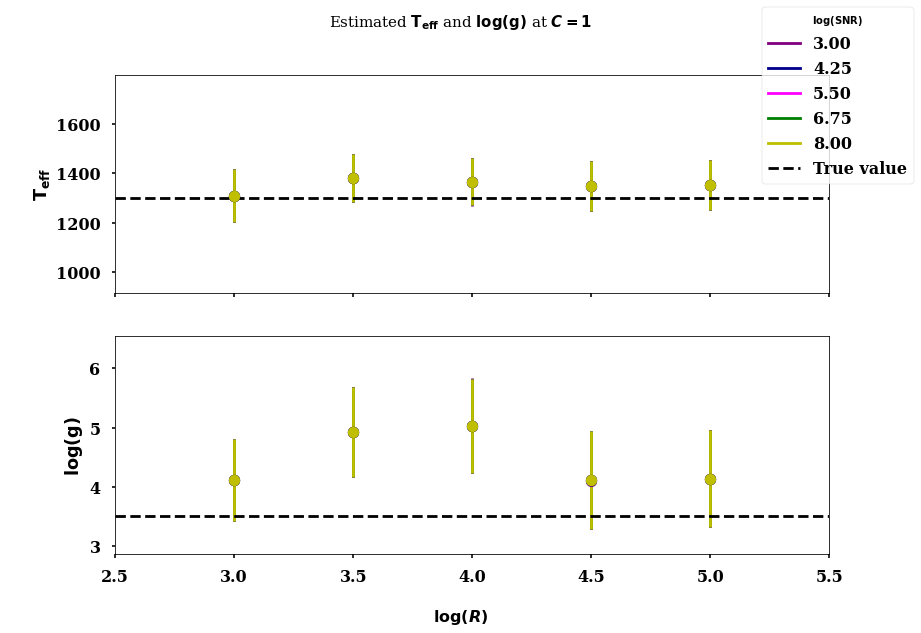
\includegraphics[scale=0.5]{images/Chapter3/char_teff_logg_C1.png}
    \caption{Caption}
    \label{fig:ceq1}
\end{figure}
Fig~\ref{fig:ceq1} shows the evolution of the estimated $\mu_{\rm{T_{eff}}}$ and $\rm{\log(g)}$ for different values of $\rm{SNR}$ and $R$.
This is a very interesting plot as the legend seems to indicate that there are different $\rm{SNR}$ values but the plot just shows one color. 
The reason for this is that the different $\rm{SNR}$ values perefectly overlap with no difference in $\rm{T_{eff}}$ and $\log{(\rm{g})}$ estimation.
The dotted line indicates the original $\rm{T_{eff}}$ and $\rm{\log(g)}$ of the exoplanet.
There are at least two interesting takeaways from this plot,
\begin{enumerate}
    \item unlike the detection matrix, the effect of $\rm{SNR}$ is absent but the contrast and perfect stellar subtraction is the biggest reason for inaccurate characterization.
    This is quite interesting because the cross correlation based detection seems to behave as a signal processing problem where with higher $\rm{SNR}$ we have perfect detection.
    However, the characterization of an exoplanet seens to behave as an astronomical processing problem whereby we need perfect stellar subtraction to achieve perfect characterization.
    \item Secondly, we notice that while the $\rm{T_{eff}}$ is perfectly characterized and indeed is defined by a nice $LL$ curve, the $\log(\rm{g})$ is not so well characterized. 
    In fact when we see the evolution of characterization accuracy we see the effect of increasing $R$ upto an $R=10^{4}$ after which this effect is take over by the presence of more absorption lines.
\end{enumerate}
The second point is fairly well defined in that based on Eq~\ref{eq:line} the $\rm{SNR_{\lambda}}$ will decrease with increasing $R$ for a fixed $\rm{SNR}$ and therefore when $\rm{SNR_{\lambda}}$ is the defining parameter to achieve a scientific goal we will see this mitigated with increasing $R$.
Characterization seems like one such goal where the best characterization seems to occur at low $R$ and high $R$ and in between we see a loss of characterization accuracy.
This particularly more evident in the case of $\log(\rm{g})$ where we work with a smaller baseline and therefore fitting a $LL$ curve is not that straightforward.

This leads us to the limitations of this method and how we expect the ML algorithms to perform better than this.
The primary limitation is the need to have a more accurate characterization method whereby the characterization matrix can be populated accurately over a larger range of contrasts.
The error bar on this characterization matrix needs to be stable over multiple $\rm{SNR}$.
However, as we have seen with the cross correlation algorithm, this is not an easy task with spectra.
Therefore,the first benchmark for ML algorithms is to identify the region in parameter space of $R,\rm{SNR}$ where we are able to characterize an exoplanet spectrum with the lowest error for $C<10^{-2}$.
This can the be followed by higher contrast characterizations if it is successful.
Note that this is subject to the condition that ML algorithms are able to make high contrast detections, i.e they are able to learn the spectral features of exoplanets at various contrasts.

\paragraph{Link between detection and characterization of spectra:\\}
An outcome of the characterization has been that in many ways the characterization accuracy is unrelated to the detection sensitivity.
However, both detection and characterization are being performed with the same spectra and the same algorithm that relies on the same spectral features.
Therefore, the question that remains to be explored is whether there is indeed any link between the two operations and if so why does this link disappear so that characterization accuracy does not improve in a lockstep manner with detection sensitivity.

Firstly the link between detection and characterization is most evident when we look at Fig~\ref{fig:nondet_char} and the equivalent detection sensitivity in Fig~\ref{fig:detmat}.
It is clear that when the cross correlation algorithm is not able to detect the exoplanet with the related $C$, the characterization accuracy is very low.
To produce the detection matrix we need to have the following relationship satisfied
\begin{equation}
    \dfrac{\rm{CC(0)}}{\sigma}\ge6
\end{equation}
allowing that the $\rm{AC}$ is mostly a constant value and the variation is the $\sigma$ and the $CC(0)$.
At $CC(0)$ there is no relative wavelength shift between the spectrum and the template.
Therefore based on \textcolor{blue}{[refer to Eq from Part II]}, we can rewrite it as ,
\begin{equation}
    CC = \sum\limits_{\lambda} F_{\rm{\lambda_{1},noisy}}M_{\lambda_1}+ F_{\rm{\lambda_{2},noisy}}M_{\lambda_2}+\cdots+F_{\rm{\lambda_{N-1},noisy}}M_{\lambda_{\rm{N-1}}}+F_{\rm{\lambda_{N},noisy}}M_{\lambda_{\rm{N}}}
    \label{eq:CC(0)expansion}
\end{equation}
and therefore we can now re-express the condition with the simplification that $\sigma = \rm{SNR}$ as 
\begin{equation}
    \dfrac{\sum\limits_{\lambda} F_{\rm{\lambda_{1},noisy}}M_{\lambda_1}+ F_{\rm{\lambda_{2},noisy}}M_{\lambda_2}+\cdots+F_{\rm{\lambda_{N-1},noisy}}M_{\lambda_{\rm{N-1}}}+F_{\rm{\lambda_{N},noisy}}M_{\lambda_{\rm{N}}}}{\rm{SNR}}\ge 6
\end{equation}
Thus, for a single entry in the detection matrix the sum of the products of the template and the spectrum has to be $\ge 6\times \rm{SNR}$.
Thus the sum of products in Eq~\ref{eq:CC(0)expansion} can be expressed as a limit of the $\rm{SNR}$ which explains why for increase in $\rm{SNR}$ we see an increase in detection sensitivity.
Thus detection sensitivity can be re-interpreted as the minimum value of the product in Eq~\ref{eq:CC(0)expansion} for which the sum of the photon values in each bin with the template is high enough to be detected.
Thus it serves as a mimimum criterion for characterization and hence for values where $\rm{SNR}<5$ the characterization accuracy will provide very unstable errorbars.
This is then the fundamental link between detection and characterization.
However, why is there not an unlimited improvement to characterization accuracy to reach perfect characterization?

In order to achieve perfect characterization we see that we need to have $C\approx1$.
In such a case we will re-write Eq~\ref{eq: true signal} as,
\begin{equation}
    F_{\rm{total},\lambda} = F_{\rm{planet},\lambda}
\end{equation}
and thus the the noisy spectrum is re-written as,
\begin{equation}
    F_{\rm{noisy},\lambda} = \textrm{random}(\textrm{PMF}(F_{\rm{planet},\lambda}))
\end{equation}
which means the noisy spectrum does not contain random values from the stellar spectrum.
Therefore, when $LL$ is calculated there needs to be higher specificity to template features to produce a deep $LL$ trough. 
This is provided only when $C\to1$ than to $C\ll 1$ which is the case for higher contrast. 
Hence, the characterization accuracy is no longer dependent on $\rm{SNR}$ but on the intrinsic exoplanetary signal present in the spectrum which is described by $C$ rather than $\rm{SNR}$.
Naturally, the characterization accuracy would not boundlessly increase as the $C$ is bound for a portion of the detection matrix.
On the other hand when we de-link it from the detection matrix we find that we are able to achieve perfect characterization.
Thus the detection and characterization are only related until the point when the characterization itself is possible but not to increase the characterization accuracy which is independent of detection.

\subsection{Why would ML algorithms be an asset if they work?}
The goals for the ML algorithms is thus two fold,
\begin{enumerate}
    \item define the limits at which ML algorithms are able to detect warm Jupiters in either context of the detection matrix or om a part of the detecton matrix parameter space and
    \item define the characterization accuracy for this part of the of the detection matrix generated by the ML algorithms.
\end{enumerate}
Before we explain why this thesis posits ML algorithms to be an asset should they work, we need to explain the reasons to test ML algorithms in the context of this chapter.
Firstly, the cross correlation algorithm as is defined in this section is limited to processing the data with one sample spectrum at a time.
The results however, have to be analyzed for more than one spectrum at a time, for instance we take $10$ noise realizations for each cell of the detection matrix and almost $50$ different templates have to be cross correlated to produce one characterization matrix is produced.
This is a perfect case for batch processing, but also statistical variations between spectra needs to be handled better than by mere averaging.
Secondly, there is no unified model for warm Jupiters that is discerned with the use of cross correlation, each template spectrum is treated as a unique spectrum whereas in reality the variation between spectra is not so unique as typified in the characterization matrix in Fig~\ref{fig:charmap-deeptrough} where $\rm{SNR_{ccf,\mu}}$ is still $>3$. 
This implies that when sufficient photons exist, all the templates provide enough similarity with test spectrum to produce a detetion.
Finally, this algorithm is still limited by the interpretation of the cross correlations through a $\rm{SNR_{ccf}}$ or $LL$ which have their own set of biases and therefore, provide only a analysis bias limited result.

This then provides the framework for ML algorithms to be, if successful, a nice alternative to the cross correlation based algorithm.
Firstly, ML algorithms are able to analyze batches of spectra and provide batch outputs and thus can populate the detection matrix much faster and with a generalized manner.
The need to train ML algorithms is a feature which allows us to train the algorithms with physical parameters that are varied.
This in turn will produce an ML algorithm that has learned the `physics' of the spectrum than working purely from the signal processing stand point.
We expect that this is more useful for astronomers, than to fine tune the cross correlation algorithms from a signal processing standpoint.
Secondly, the fact that the biases of ML algorithms are well quantifiable, by means of receiver operating characteristic curves for example, means that the algorithmic biases can be well understood. 
The statistical fluctuations can also be well quantified  with the help of a large and varied dataset.
This means we don't rely only on averaging the results but will be able to limit these statistical fluctuations by controlling the variance in the data.
Finally, the use of ML algorithms will constitute a fast, robust and reliable way to detect and characterize the spectrum simultaneously and we will use the parameter space from the chapter to train the ML algorithms on.
\chapter{Development and performance of the ML algorithms}
\label{chap:III.5}
In the previous chapter we presented the cross correlation based detection and characterization algorithms along with the results for a clearly defined parameter space.
For the training, validation and testing of ML algorithms in this chapter we continue use the same data set as in the previous chapter.
The advantage of being able to generate a practically unlimited number of spectra allows us to extend our scope to try to cover as much of the top five rows of the detecton matrix as possible.
We confine ourselves to using the highest $\rm{SNR}$ cases for two reasons,
\begin{enumerate}
    \item the top rows allows us a a full range of contrasts to test if the faintest exoplanet detected by the cross correlation algorithm is still reachable by the ML algorithms
    \item and to ensure that the lack of photons does not limit our ability to test ML algorithms in the field of high contrast exoplanet detection.
    This would serve as the best opportunity to test the ability of ML algorithms with a large observing baseline.
\end{enumerate}
The results of that chapter will serve as the basis to develop the ML algorithms used in this chapter.
In this chapter, we describe the ML algorithms that are used for this part in my thesis. 
The goals of this chapter are the following,
\begin{enumerate}
    \item describe the parameter space and the motivation for the use of parameter space based on the results of the previous chapter. This will form the "data" description in this chapter.
    \item Describe the motivation and development of the ML algorithms that will be used in this part of the thesis. The background description of these algorithms are assumed from §\ref{chap:III.2}. 
    \item Describe first the results of the cross correlation algorithm evaluation using the confusion matrices described in §\ref{chap:III.3} followed by the algorithm evaluations of the ML algorithms used.
    \item Finally, we end this chapter with a discussion on why the ML algorithms were not used in further science evaluations and its consequences for the use of spectra with ML algorithms.
\end{enumerate}
\begin{comment}
Describe how these case studies were chosen and why they are relevant to the study.
What do we learn when they fail or pass
In order for ML to be considered \textit{more effective} it needs to be able to make detections at higher contrast than $(C\approx10^{-2}$ for a $\rm{SNR}\le10^4)$ across $R$.
\end{comment}
\section{Experimental parameter space selection and testing they hypotheses}
The parameter space begins with identifying the combination of $(R,\rm{SNR},C$ for the purposes of training, validation and testing the ML algorithms.
The goal of this exercise is to primarily divide the parameter space into two broad categories,
\begin{enumerate}
    \item identify cases that would serve as the basis to evaluate the ML algorithms and "fail fast" if the algorithms need to be marked as not appropriate for this purpose. 
    A failure to make the appropriate false positive bar would lead the algorithms trained to be marked as inappropriate for this problem. 
    A pass at this stage using confusion matrices indicates that ML algorithms are eligible to check for higher contrast cases which will allow us to compose the detection matrix.
    \item The second category would be the highe contrast cases where the contrast is high enough that only higher $\rm{SNR}>10^{4}$ will be able to detect the exoplanets in these spectra.
    This second category is the tipping point to define if ML algorithms can indeed be compared with the cross correlation algorithm.
\end{enumerate}
In this section we will begin with describing the problem statement that will be used with ML algorithms first for detection and then for characterization.
The hypotheses statements still remain valid and therefore they have to be tested with ML algorithms.
We will follow this with describing the parameter space that will be chosen for each category and both the scientific and data challenge posted by this parameter space.
\subsection{Adapting ML algorithms to test the detection hypothesis}
In order to test the detection hypothesis, the first step is to pose the problem accurately so that an ML algorithm can be used to test the hypothesis.
The detection hypothesis was tested using the cross correlation algorithm by inferring the conditions (namely $R$ and $\rm{SNR}$) that are necessary to achieve perfect detection (namely detecting an exoplanet at $C=10^{-6}$).
The condition for detection was set at $\rm{SNR_{ccf}}\ge 6$ due to its low false positive rate,
The $\rm{SNR_{ccf}}$ is defined as the single parameter that will allow us to determine the fitness of the exoplanet to be detected.
Thus, we have shown that with the detection hypothesis can be proven with the use of the a detection criterion parameter ($\rm{SNR_{ccf}}$), the detection criterion ($\rm{SNR_{ccf}}\ge 6$) and the detection matrix.
The detection parameter will continue to remain the contrast at which we meet the detection criterion when applied to the detection criterion parameter.
Following this recipe, we will also define the first two criteria for ML algorithms when validating the detection hypothesis. 
The detection matrix remains the same to be used for both the ML algorithms and the cross correlation algorithm.

\paragraph{Detection criterion parameter:\\}
The ML algorithms are able to provide two types of outputs as discussed in \Cref{chap:III.2} namely categorical or a regression output.
We explained that when the classes of the output are well known the categorical or classification problem is best chosen.
In this case we can have two possibilities for each spectrum, either it contains features for an exoplanet or it does not contain these features. 
These categories are of course not well separated because a high contrast exoplanet may not be detectable at all.
This was the reason for the detection hypothesis, which states that there are indeed conditions where the exoplanet is detectable with an appropriate algorithm.
We used the detection matrix to find the conditions where the parameter space separates the spectra as having exoplanet features and therefore detectable even at the highest contrast and not having exoplanet features and therefore not detectable.
We use this idea to define the problem of ML algorithms as a classification problem. 
Given the right conditions the spectra should be clearly separable as containing an exoplanet or not containing one.
The detection criterion parameter, therefore is a class of whether an exoplanet exist $y=1$ or not $y=0$ and therefore we re-express Eq~\ref{eq: true signal} and Eq~\ref{eq:insertion} as 
\begin{eqnarray}
    C_y =& y\times C\\
    F_{\rm{planet},\lambda,new} =& C_y\times F_{\rm{planet},\lambda,old}\times \rm{SNR}^2\\
    F_{\rm{total},\lambda} =& (1-C_y)F_{\rm{star},\lambda,new} + F_{\rm{planet},\lambda,new}
    \label{eq:ML_detect_eqn}
\end{eqnarray}
The rest of the equations continue as before from §\Cref{chap:III.3}.
We are thus able to generate spectra to be used as training for ML algorithms.
As with any classification algorithm, the value of $y$ is universally only $0$ or $1$ but lies on a sigmoid curve such that when the exoplanet features exist $y\to 1$ and when they don't exist $y\to0$.
Therefore, a second criterion to the detection criterion parameter is necessary such that we can quantize $y$.We choose the criterion as $y =1$ when $y>0.5$ and $y=0$ when $y\le 0.5$.

In order to understand how the spectral features of the noisy spectrum in \Cref{eq:insertion} evolves with different contrasts we present a series of plots where the contrast is reduced and this produces a higher $\rm{SNR_{ccf}}$.
Note that the $\rm{SNR_{ccf}}$ is sensitive to changing $C$ exponentially, whereas it is related to $\rm{SNR}$ linearly.
\Cref{fig:compare-specsnr=5.24} shows a spectrum generated with a $\rm{SNR}$ with two classes, $y=0$ in pink and $y=1$ in green. 
The topmost plot is a sample template spectrum re-sampled to the spectral resolution $R=1000$.
The bottom most plot shows the cross correlation strengths as a function of velocity of both the pink and the green spectra.
Note that visually, it is not possible to tell apart the green and pink spectra, but the cross correlation algorithm is able to make this distinction.
In order to also illustrate a case where the difference between the pink and green spectra is stark, we choose a very high $\rm{SNR}$ and low $C$ in \Cref{fig:compare-specsnr=3000}.
We can clearly see the shape of the template and its specific features in the K-band and H-band.
\begin{figure}[ht]
    \centering
    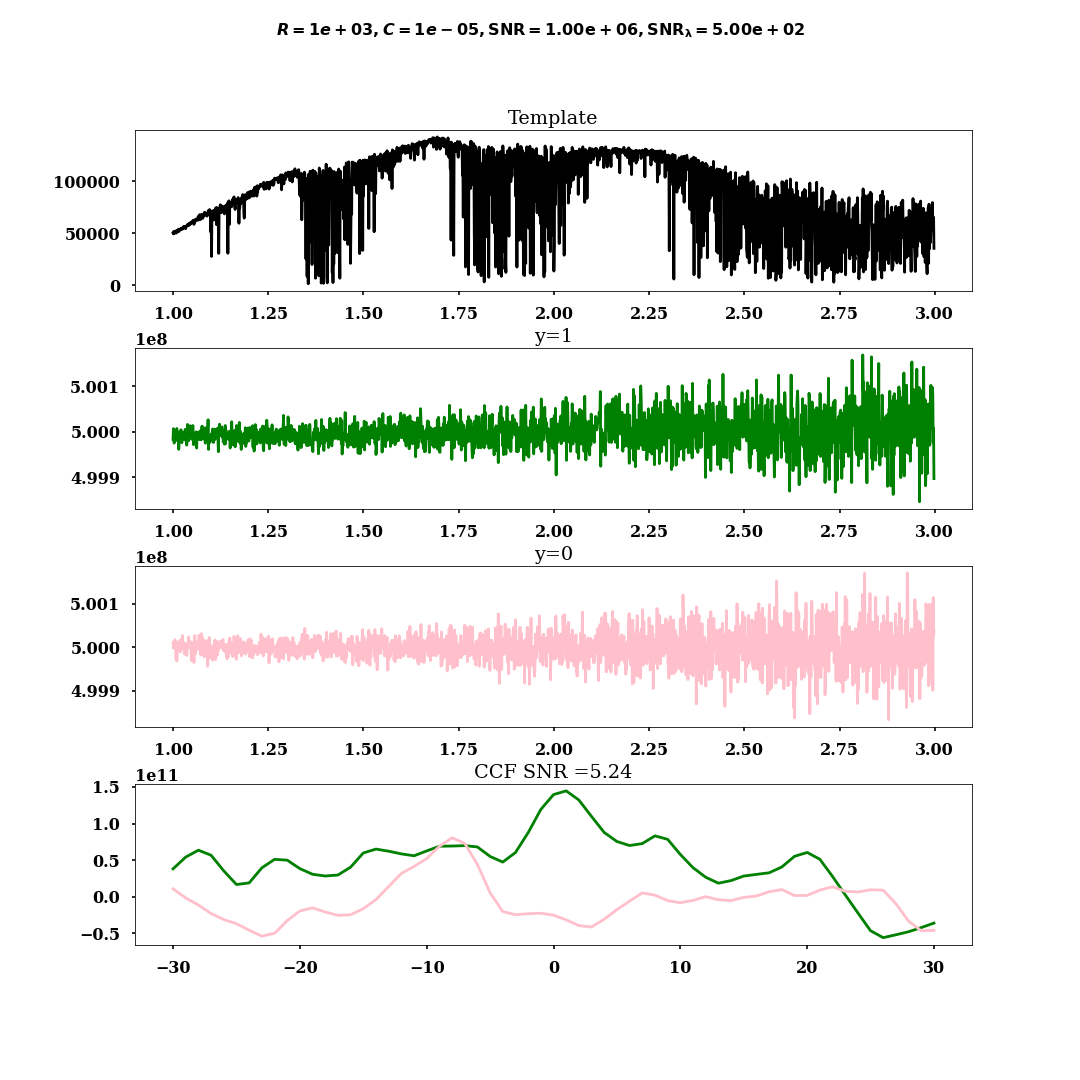
\includegraphics[width=\textwidth]{images/Chapter3/feature_compare_ccf_snr_5.24.png}
    \caption{Caption}
    \label{fig:compare-specsnr=5.24}
\end{figure}

\begin{figure}[!hb]
    \centering
    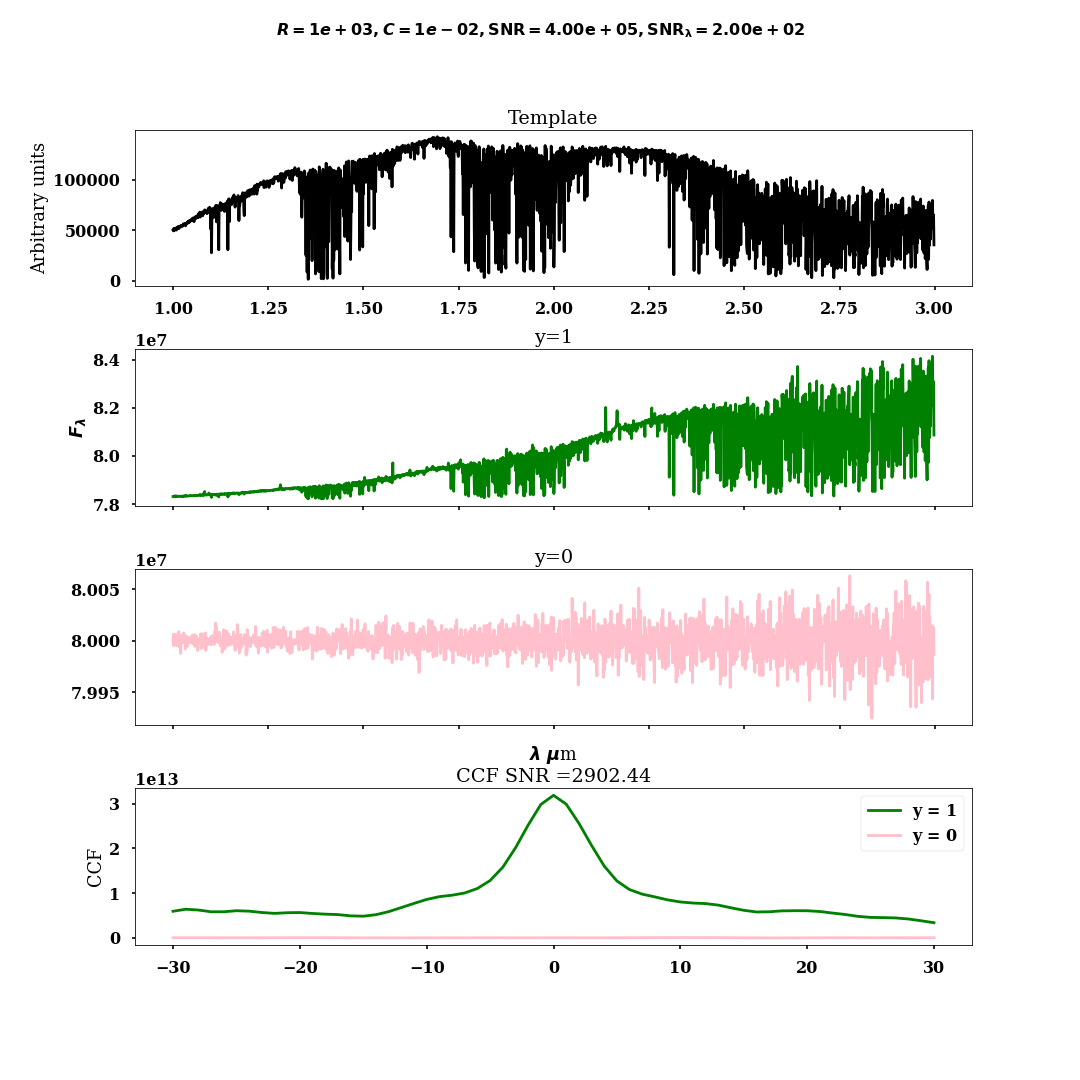
\includegraphics[width =\textwidth]{images/Chapter3/feature_compare_ccf_snr_2902.44.png}
    \caption{Caption}
    \label{fig:compare-specsnr=3000}
\end{figure}
Thus, we have the detection criterion parameter $y$ that will serve as the prediction parameter for the ML algorithms with the spectra being inputs.
\paragraph{The detection criterion:\\}
The final part of adapting ML algorithms is to establish the detection criterion that needs to be met in order to test the detection hypothesis.
As stated above when the output of the ML algorithm is between $0.5$ and $1$, we quantize the output to mean the predicted value of $y$ ($y_{\rm{pred}}$) which will then be used to populate the detection matrix.
The detection matrix as constructed using the cross correlation algorithm was built by simultaneously analyzing a large number of spectra and then populating the matrix with the results of this analysis.
For ML algorithms, as explained in \Cref{chap:III.2}, we need to train, validate and test these algorithms taking care to not overfit the data.
A lot of the overfitting will be taken care by providing sufficient variance in the data described in \Cref{subsec:paramspace}.
For the purposes of describing generating the detection matrix, it is sufficient to say that we generate over $15000$ spectra in total to produce the training, validation and test datasets.
The detection criterion still remains the detectable contrast $C$ and we will establish the mean contrast that is detectable for a range of $\rm{SNR}$ and $R$, once again chosen with a criterion similar to \Cref{fig:parspace-1}.

In order to now establish the detection criterion for a specific parameter values we proceed with the following steps,
\begin{enumerate}
    \item we first generate a large number of spectra with one specific template with variations being made in $\rm{SNR}$ and $C$ but a fixed $R=1000$. We divide these spectra into training, validation and test datasets.
    We then train the ML algorithms with the training  datasets and use the validation dataset to fine tune the following parameters, the learning rate gradient, the momentum, the mix of contrasts involved and the hyper parameters of the ML algorithm being used.
    The first two are changed continuously during training depending on validation error, but the mix of contrasts is changed so that the validation error is $\approx 10^{-5}$.
    We then test the algorithms with the test data by producing confusion matrices.
    \item When the false positive rate is low enough, we proceed to generate fresh spectra in the contrast ranges used for training (no matter the validation error) and compute the confusion matrices for these. 
    These will be exactly the same as the test confusion matrices but to rule any statistical uncertainties we produce fresh spectra.
    We use these confusion matrices and identify the highest contrast where we can produce a confusion matrix so that the true positive rate $>0.5$ and the false positives produces are $1$ for $10000$ spectra.
    \item We then perform this operation for each of the $\rm{SNR}$ in the parameter space and identify $C$ to populate the detection matrix.
\end{enumerate}
Note that we will start with highest $\rm{SNR}$ to ensure that we rule out the possibility of that ML algorithms fail the detection hypothesis.
\subsection{Adapting ML algorithms to test the characterization hypothesis}
The characterization hypothesis is tested using the characterization matrix.
As with detection matrix, the characterization matrix is populated by the characterization parameter which was the $LL$ in \Cref{chap:III.4}.
The characterization parameter could have also been $\rm{SNR_{ccf}}$, but for reasons explained in \Cref{chap:III.4} we use $LL$ which is the negative square of the $\rm{SNR_{ccf}}$.
We don't have any known literature which connects the value of $y_{\rm{pred}}$ and any Gaussian distributed parameter that will allow us to derive a $\chi^{2}$ error bar.
Therefore, in this subsection we will briefly describe two different strategies to produce a characterization parameter and the merits and demerits of both. 
It is to be noted that if the ML algorithms fail the detection hypothesis, there is not enough evidence that they will be able to test the characterization hypothesis.

As already explained in \Cref{sec:classifcation and regression}, supervised algorithms are either classification or regression algorithms. 
In practice this means that either the output of the ML algorithm is completely unbounded or is bounded to remain between $0$ and $1$.
Since we don't have any prior art in this regard, we postulate using both regression and classification as approaches to produce the characterization matrix.
The caveat of this section is that neither of these approaches were validated as ML algorithms failed the detection hypothesis, but this section is evidence of clear experimental planning before we explain the ML algorithms.
\paragraph{Use of regression to compute the characterization parameter:\\}
When using regression to compute the characterization parameter, we directly compute the $\rm{T_{eff}}$ and $\rm{\log(g)}$ from the ML algorithms.
The question is how doe we compute the error bars on these quantities.
We first define the output of the ML algorithm to be two quantities i.e $\rm{T_{eff}}$ and $\rm{\log(g)}$ for each spectrum.
We then use an appropriate error function such as the mean square error to compute the error on these quantities.
As the mean square error will be the quantity minimized, we will have the minimum mean square error on these quantities separately.
However, in order to compute the true error bar we had posited the following steps,
\begin{enumerate}
    \item generate a large number of spectra for a fixed value of $\left(C,R, \rm{SNR}\right)$ so that each spectrum represents only a different noise realization. Based on our results in \Cref{sec:char error bars} and \Cref{sec:removal of stellar}, it is clear that the biggest effect on characterization error bars is the stellar contamination. 
    \item fit a non-parametric curve to the results produced from these spectra to compute the means and standard deviations.
    \item this will result in one mean and standard deviation for both $\rm{T_{eff}}$ and $\rm{\log(g)}$ for each combination of $(C,R,\rm{SNR})$ and
    \item finally, we will generate characterization matrices for each value of $C,R$ for several $\rm{SNR}$ to produce a result akin to \Cref{fig:perfectchar}.
\end{enumerate}
This can then be used to verify that the error bars are quantifiable for specific values of $C$.
The advantage of this technique is that we can directly regress to the value of $\rm{T_{eff}}$ and $\rm{\log(g)}$.
The disadvantage of this method is that it is possible the distribution of $T_{eff}$ and $\rm{\log(g)}$ does not lend to accurate error or mean calcuation, in which case it would be pointless. 
This type of regression does not lend to clean graphical qualification of the performance of different templates.
Hence we will also explore a slightly different way of quantifying the mean and standard deviation
\paragraph{Design of a characterization matrix with a logistic characterization parameter:\\}
The goal of the characterization matrix is to compute the mean $\rm{T_{eff}}$ and $\rm{\log(g)}$ and their uncertainties.
We also like a nice graphical way that can describe the similarities between different templates.
To achieve this we define a new parameter $p$ such that,
\begin{equation}
    y_{\rm{pred}} = p
    \label{eq:p-ypred}
\end{equation}
The distribution of $p$ for a single spectrum is \Cref{fig:sample charmat}.
\begin{figure}
    \centering
    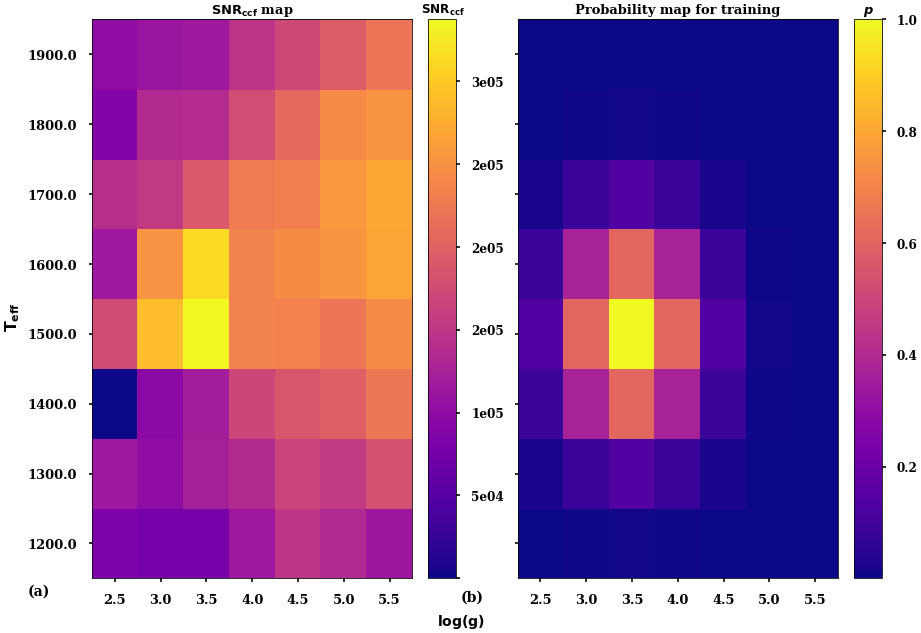
\includegraphics[width=\textwidth]{images/Chapter3/subplots_snr_p.png}
    \caption{Caption}
    \label{fig:sample charmat}
\end{figure}
For every spectrum, we will have a characterization matrix with different $p$ values.
The $p$ values are distributed as a 2D Gaussian centered on the $\rm{T_{eff}}$ and $\rm{\log(g)}$ of the template of the exoplanet.
A sample map is shown in \Cref{fig:sample charmat} alongside a characterization map with $\rm{SNR_{ccf}}$ as the characterization parameter.

We posit that a ML algorithm can learn to recognize feature strengths that vary as a Gaussian centered around the inserted template.
The standard deviation of this Gaussian will give us uncertainties of both $\rm{T_{eff}}$ and $\rm{\log(g)}$.
We will use a logistic error function such as the categorical cross entropy to minimize the training error.
We will generate large number of spectra with constant $\rm{SNR},R$ and slightly varying $C$ so that we can have some variance in the data.
We will automatically produce these characterization matrices and train the ML algorithms to produce the same matrices for every spectrum.
The advantage of this approach is that we get a characterization matrix which has a parameter that can be related to detection.
We can also get a very good visual reference for large number of spectra and verify that the error bar is consistent for different types of spectra.
Finally, these matrices allow us to infer whether ML algorithms are able to distinguish between templates in one glance.
The disadvantage of this approach is that there is no evidence that the output of ML algorithms will obey this distribution.
There is also little evidence to show that \Cref{eq:p-ypred} holds true for large number of spectra with any bounding condition.

\subsection{Parameter space selection}
\label{subsec:paramspace}
The parameter space selection is simplified by the tests performed using the cross correlation algorithm and the resulting detection and characterization matrices.
There are two takeaways from these tests that we will continue to work with while choosing the parameter space to train, validate and test the ML algorithms,
\begin{itemize}
    \item the $\rm{SNR}$ is the most important parameter to validate the detection hypothesis, in turn this means that for the highest $\rm{SNR}$ the detection hypothesis has the highest chance of being validated for all contrasts concerned.
    Note that this does not preclude that ML algorithms will automatically perform exactly as the cross correlation algorithm has performed, but merely chooses the best possible chance for ML algorithms to succeed.
    \item Secondly, it is clear that detection and characterization are linked through the contrast, where we know that if the contrasts are low and $\rm{SNR}$ we are able to perform simultaneous detection and characterization. But what needs to be seen if ML algorithms are able to consistently find the spectral features for different contrasts to convince us to use them to characterize spectra.
\end{itemize}
Point 2 thus raises an important question, i.e will ML algorithms work on both the low and the high contrast space.
With this in mind, while keeping $10^{5}>\rm{SNR}>10^{6}$, we divide our parameter space into a low contrast parameter space corresponding to $C>10^{-3}$ and a high contrast parameter space $10^{-3}>C>10^{-4}$.
\paragraph{Low contrast parameter space:\\}
The low contrast parameter space is defined where the contrast is between $10^{-2}>C>10^{-1}$.
As described earlier, we choose the highest $\rm{SNR}$ between $10^{5}>\rm{SNR}>10^{6}$ to give the ML algorithms the best chance to train.
We fix the $R=1000$ for two reasons, firstly that there has not been significant evidence to show that $R$ has much impact on the detection or characterization of an exoplanet particularly when testing our hypotheses.
Secondly, higher $R$ means higher number of bins and consequently larger memory and computational requirements.
Therefore, we choose a low $R$ to test our hypotheses with ML algorithms.
As stated before, we generate a large number of spectra based on \Cref{eq:ML_detect_eqn}.
In order to keep this fair we also validate the spectra by running them through the cross correlation algorithm and setting a $\rm{SNR_{ccf}}>5$ to set the $y_{\rm{pred,ccf}}$.
We sample the parameter space such that the distribution of spectra is fully within the sample space.
To illustrate this we plot the spectra generated based on the parameter space, such that a single spectrum generated with a combination of $\rm{SNR},C$ is represented as a single point in \Cref{fig:trained_sample space}.
The sample space is filled with three colors pink points corresponding to $y=0$, black corresponding to spectra undetected by the cross correlation algorithm ($y=1$) and green points corresponding to those that are detected. 
The absence of black points in \Cref{fig:trained_sample space} shows that there are no spectra which are missed by the cross correlation algorithm.
This plot also illustrates that the parameter space is well filled and the balance between $y=0$ and $y=1$ spectra is fairly even.
\begin{figure}[!h]
    \centering
    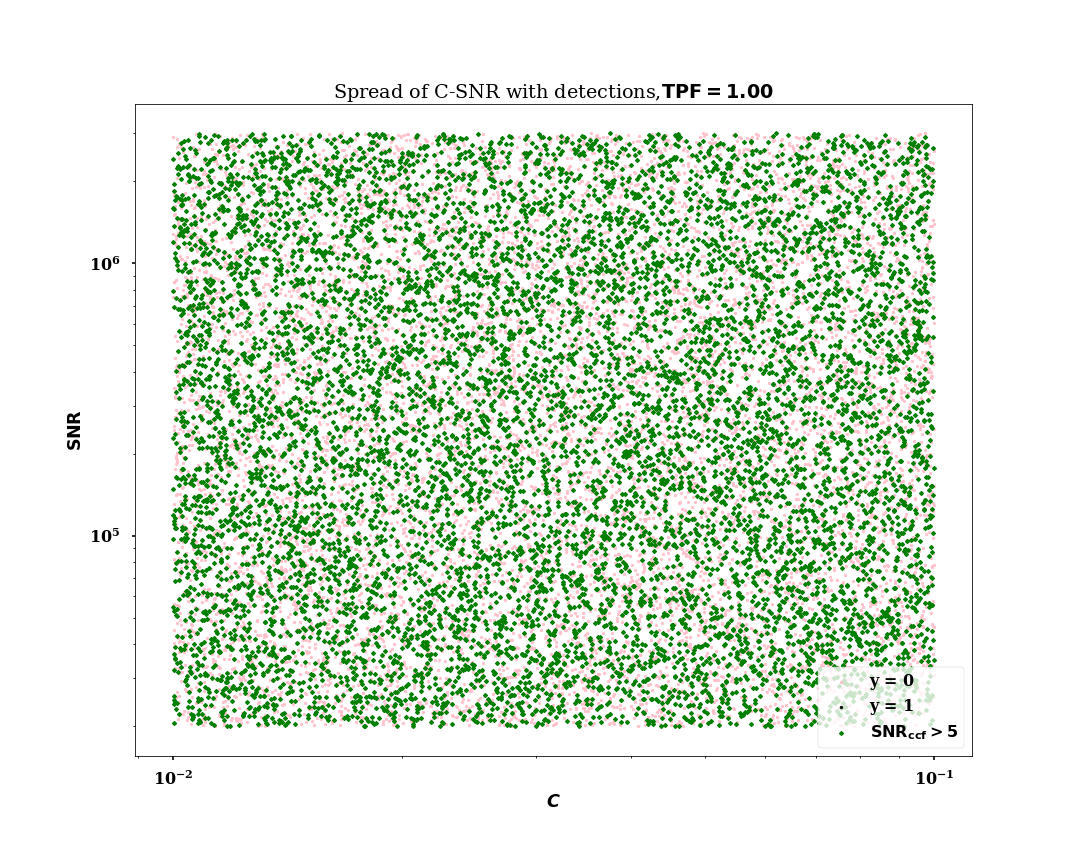
\includegraphics[scale=0.4]{images/Chapter3/samples_trained.png}
    \caption{Caption}
    \label{fig:trained_sample space}
\end{figure}
\paragraph{high contrast parameter space:\\}
For the high contrast parameter space we choose a contrast range of $10^{5}>C>10^{3}$. 
In principle we could choose the highest contrast, but we also wanted make a parameter space where the true positive rate for the cross correlation algorithm was slightly higher than $0.5$.
This gives us confidence that majority of the spectra indeed contain features that are detectable by a `classical' algorithm. 
At the same time there are a few samples that provide a `challenge' to the ML algorithms to detect.
A similar plot to \Cref{fig:trained_sample space} is used to depict the samples drawn from this parameter space.
In \Cref{fig:untrained_sample space} we see some black dots filling up $\approx 30\%$ of the parameter space, whereas the rest of the parameter space is covered by green dots.
Note that $\rm{SNR_{ccf}}>5$ is a somewhat `high bar' to ensure we don't end up with a high false positive rate and does not mean that those spectra which deliver a $\rm{SNR_{ccf}}\approx 4.5$ are non detectable or that they don't contain features that are detectable.
\begin{figure}
    \centering
    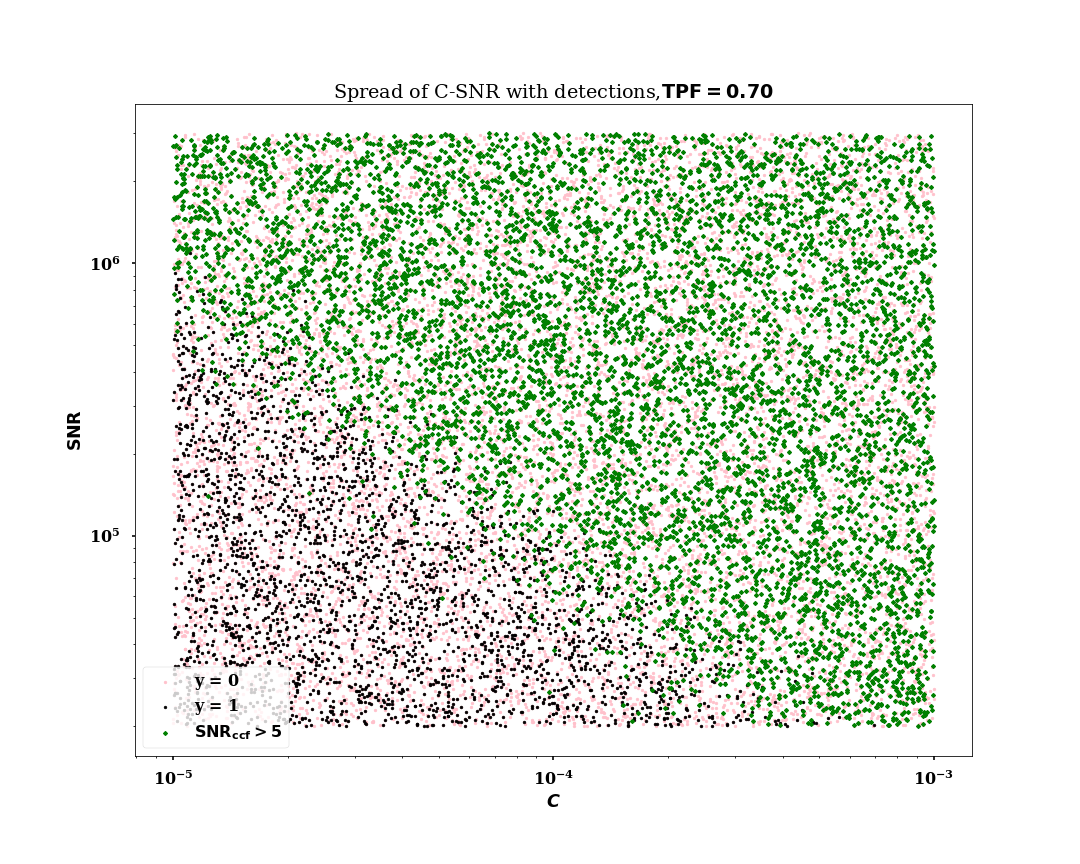
\includegraphics[scale=0.4]{images/Chapter3/samples_nontrained.png}
    \caption{Caption}
    \label{fig:untrained_sample space}
\end{figure}

When reporting the results we will make this discrimination of high and low contrast parameter spaces as the results also are neatly divided in between these parameter spaces.
A final word on this parameter space is that while the contrast cut off between the spaces is somewhat arbitrary, there is a clear scientific justification for dividing these contrasts.
Firstly, the low contrast cases are what would be really bright targets and therefore, if known they would correspond to the first set of targets that would be used to test new instruments and algorithms.
These would also correspond to targets whose properties of $\rm{T_{eff}}$ and $\rm{\log(g)}$ are well defined and so they can be well quantified and verified.
In principle, therefore this parameter space represents some of the well defined targets.
Secondly, the high contrast space is that which is typical of targets that are the most numerous in the high contrast imaging.
Therefore, this represents the targets that ML algorithms will most likely be presented with and therefore the performance on this parameter space is the test of failure of ML algorithms. 
It is on this parameter that we need to quantify the performance of ML algorithms on.
\section{ML based algorithms}
ML algorithms come in different flavours and types and a brief introduction to this was presented in \Cref{chap:III.2}.
As stated earlier, this thesis primarily works with supervised classifiers to test the detection hypothesis and we could choose supervised classifiers or regressors to test the characterization hypothesis.
As we shall see in the  \Cref{sec:ML results} the performance of ML algorithms did not provide us with the confidence to try out characterization strategies.
Therefore, this section will primarily discuss the algorithms used for testing the detection hypothesis.
However, we would be remiss in assuming that these algorithms could not be adapted to test the characterization hypothesis.
We will, therefore, also suggest ways to adapt this algorithm for the characterization case.
We will discuss later the ways that spectra could be used directly with ML algorithms that is out of the scope of this thesis but could be tried out easily in the future with the framework provided by this thesis.

\textcolor{red}{This is a very crucial paragraph which justifies how what I have done different from 2020 Fisher.
Note there are indeed very many similarities and it is possible this is one of the weakest points, that it is not fair to expect any characterization from ML as the Fisher paper exactly reports this.
I aim to justify this as 1. I use detection to test if this method can be used with HCI data 2. we then will move to characterization iff we are able to compose the detection matrix with ML algorithms.}
As described in \Cref{chap:III.2}, supervised classifier algorithms come in different types, in this thesis we use ensemble and deep learning algorithms.
The goal of trying two different kinds of algorithms is to verify whether a) are results consistent over different types of algorithms and b) whether any kind of algorithm offers an advantage to this type of analysis.
As stated before \cite{2020Fisher} has explored the use of random forests and deep learning algorithms with cross correlation data, which are similar in the sense that they are also large 1D vectors.
However, the same algorithms have not worked with spectra directly, when ML algorithms have been used to constrain the metallicity and temperature directly from the spectra.
There are two fundamental differences from how we are posing the problem,
\begin{enumerate}
    \item firstly, we pose this problem as a pure detection problem where we are detecting an exoplanet as an inference based on the presence of an ensemble of exoplanet features in the spectra and
    \item secondly, the characterization part of the problem is essentially an extension of the detection where we identify the closest template to the one that is present in the data and use that to infer the properties of the exoplanet.
    \end{enumerate}
    In addition we choose the parameter space of the spectra after carefully whetting it by running them through the cross correlation algorithm. Finally, we will use the ML algorithms to first the detection hypothesis to define if ML algorithms are able to validate it before validating the characterization hypothesis.
Our ML detection and characterization algorithm is a three step algorithm,
\begin{enumerate}
    \item in the first step we conduct the data generation and normalization where we generate the data specified by the parameters of $C,R,\rm{SNR}$ this is followed by,
    \item the passing of the spectra through the ML algorithms which either detect or could produce a characterization output and finally,
    \item this is terminated with a analysis step which is usually either a confusion matrix where we know the truth values or a threshold application.
\end{enumerate}
The final step is the scientific outcome that is relevant to this thesis.
\subsection{Data generation and pre-processing}
We first generate data as in \Cref{fig:trained_sample space} for the low contrast parameter space.
We choose a range of templates to initially begin with in order to minimize the chance that the ML algorithm will memorize wavelength features specific to the template.
As we produce these spectra, we also run them through cross correlation based detection algorithm to ensure that the statistics are inline with \Cref{fig:detmat}.
We generate a total of $12000$ spectra within this parameter space. 
We divide these spectra into $\approx10000$ spectra for training, $\approx 2500$ for validation and $500$ for testing.
We report each of these results in \Cref{sec:ML results}.
Our partition of data follows the $80\%$ for training, $15\%$ for validation and $5\%$ to test.
The idea being that the validation examples will allow us to provide a rigid buffer against overfitting, at the same time ensuring that we have enough samples to assess if it is underfitting.
The test is meant to serve as a failsafe to avoid overfitting the training and validation.
Once spectra have been generated, divided into the sample datasets, we first normalize them using the standard scaler which is expressed as,
\begin{equation}
    F_{\lambda,\rm{norm}} = \dfrac{F_{\lambda,\rm{noisy}}-\mu_{F_{\lambda,\rm{noisy}}}}{\sigma_{F_{\lambda,\rm{noisy}}}}
\end{equation}
where $\mu$ and $\sigma$ are the mean and standard deviations of the spectrum. 
\subsection{ML algorithms}
This section will describe the development of the different ML algorithms starting with the random forest on the basis of the steps of generating data, training the algorithms and validating and testing them.
\paragraph{Random forests:\\}
As stated earlier in \Cref{chap:III.2},among the ensemble algorithms, random forests have the properties that are most suited to deriving inferences from large vectors.
We pose the problem as classification problem to the random forest where the input is a normalized input spectrum and the random forest attempts is trained to classify the result as $y=0$ or $y=1$.
We then start with the standard number of $1000$ trees in the random forest and other default parameters of the \textsc{sklearn} implementation.
We then progressively increase the number of trees in the forest until we have similar confusion matrices for the training and validation matrices.
We will describe the different matrices in results section, but the goal is to have $0$ false postives and true positive fraction $>0.5$.
We found that the best validation matrix is achieved for $3000$ trees.
We also found that increasing the number of forests, minimum node split etc. had little to no impact on the training loss. 
\paragraph{MLP:\\}
In this thesis, we use the MLP to verify whether adding a depth dimension allows our ML algorithm to generalize better and test the detection hypothesis.
We started with small neural networks and grew it depth wise, slowly adding depth as the results with validation data on the low contrast dataset. 
We finally settled on a $11$ layer architecture where the activation function is a "Rectifying Linear Unit (ReLU)" with the exception of the last layer which has a sigmoid output to predict the class or another ReLU to predict the value.
As before, we first produce spectra which can be processed with the cross correlation algorithm.

We iteratively changed the number of neurons in each layer based on the output of the validation step. 
Based on the confusion matrices generated from the low contrast dataset, we settled on the following configuration that allowed us to produce identical train, validation and test confusion matrices, 
$\left[6000,3000,1500,600,300,150,60,40,30,20,1\right]$ for each layer starting from the input to the output class.
\paragraph{Autoencoders:\\}
An autoencoder, as stated in \Cref{chap:III.2}, has been used effectively in classifying stellar spectra.
The sparse reconstruction of an autoencoder seems quite ideal for spectra which contain distinct features in just a few wavelength bins whereas the rest of the bins are mostly noise.
In our case we use the full wavelength configuration and thereby contain absorption features in each wavelength.
In order to use this idea we built an autoencoder with small amount of layers to begin with and then built it up as the results of the validation confusion matrix improved for the low contrast case.
We settled on an architecture that consisted of $6$ encoding and $7$ decoding layers each layer had a ReLU activation.
In addition, there was an input layer with ReLU activation with as many neurons as the input vector size $\rm{N}$ and the output was a single sigmoid neuron to classify the spectra.
The autoencoder had a mirrored architecture for the encoding and decoding layers.
We start the encoding layer with $1024$ neurons, sequentially dividing the number of neurons by $2$ until we reach $32$ neurons.
The decoding layer then starts with $32$ neurons and ends with $1024$ neurons and one last layer of the same size as the input layer and finally terminating with the output sigmoid.

For both of the deep learning algorithms the loss that we use is the binary cross entropy loss with the ADAM optimization routine.
The output of all of these algorithms are subject to two evaluations 1. being the basic algorithmic evaluation where the robustness of the ML algorithms to reproduce the results of cross correlation algorithms will be tested 2. being the scientific validity by constructing the detection matrix using the ML based algorithm.

\section{ Experimental results}
\label{sec:ML results}
The experimental results section of the ML experiments will contain three parts,
\begin{enumerate}
    \item we will first describe the results of the performance of the cross correlation based algorithm to establish the benchmark of algorithmic performance and to be convinced that the data generated for these experiments were indeed reasonable for the experiment goals.
    \item Then we will describe the low contrast results produced by the ML algorithms using confusion matrices
    \item and then finally we will end with describing the results produced by ML algorithms when they were trained with high contrast data.
\end{enumerate}
The goal of this section is to clarify the limited scope of ML algorithms but also to showcase that using them in the limited manner will produce somewhat reliable results.
\subsection{Performance of the cross correlation algorithm as a classifier}
The performance of the cross correlation based detection algorithm is defined by the number of false positives and the true positive rate.
The true positive rate is given by,
\begin{equation}
   \rm{TPR} = \dfrac{TP}{TP+FN}
\end{equation}
where $\rm{TP}$ is the total number of $y=1$ cases that produce a cross correlation with $\rm{SNR_{ccf}}>5$,
$\rm{FN}$ are the total number of $y=1$ cases that produce a cross correlation with $\rm{SNR_{ccF}}<5$.
The $\rm{FP}$ are the $y=0$ cases that produce $\rm{SNR_{ccf}}>5$.
We run about $10000$ spectra through this algorithm to determine the number of $\rm{FP}$s produced.
\begin{figure}[!ht]
    \centering
\begin{subfigure}{0.4\textwidth}
    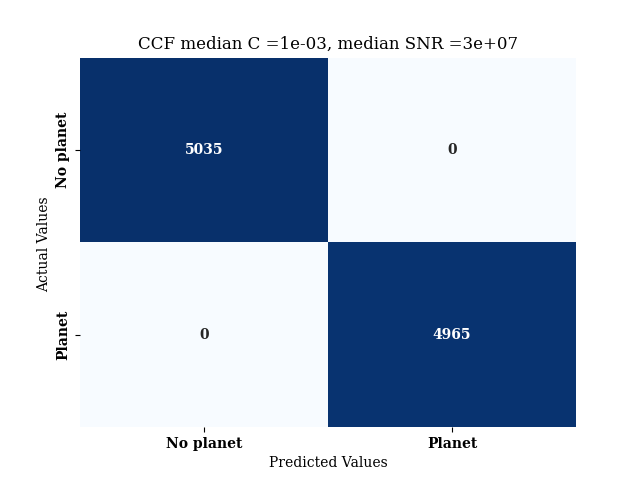
\includegraphics[scale =0.5]{images/Chapter3/confusion_ccf_1e-04_cmax_1e-02_dsnrmin_1e+07_dsnrmax_1e+08.png}
    \caption{Caption}
    \label{fig:ccf_cm}
\end{subfigure}
\hfill
\begin{subfigure}{0.4\textwidth}
    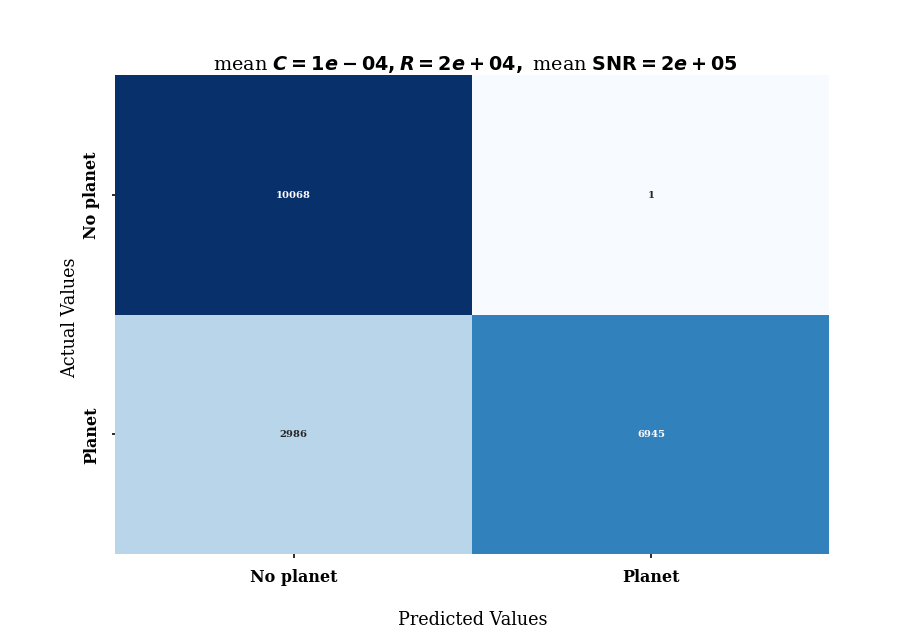
\includegraphics[scale=0.28]{images/Chapter3/ccf_cm_cmin_1e-5_cmax_1e-3_snrmin_1e5_snmax_1e6_R_20000.png}
    \caption{Caption}
    \label{fig:high contrast-ccf cm}
\end{subfigure}
\caption{CCF results}
\end{figure}
\Cref{fig:ccf_cm} shows a sample confusing matrix when generating a sample set with a median $C=10^{-3}$ with lowest $C=10^{-4}$ and the highest $C=10^{-2}$ and median $\rm{SNR}=10^{7}$.
In this case we have $\rm{FP}= 0$ and $\rm{TPR}=1.0$.
We also observe a case at higher contrast with mean $C=10^{-4}$ in \Cref{fig:high contrast-ccf cm} where we see that while with a $\rm{FP}=1$ we have a low number of false positives for $15000$ examples; we have a low $\rm{TPR}=0.67$ owing to both the higher contrast and the lower $\rm{SNR}$.
Note that for both figures, we are well beyond the detection limit based on \Cref{fig:detmat}.
However, this exercise is meant to illustrate the different ranges of training examples that are used with the ML algorithms.
Since higher $\rm{SNR}$ are more amenable to detection over a range of contrasts, they are the initial range of $\rm{SNR}$ that will be used for training.
\subsection{Low contrast results}
The low contrast performance was sequentially tested with random forests, MLP and autoencoders.
We will present the results here from the test set, the contrast ranges of $10^{-1}$ to $10^{-3}$ which is the "low contrast" region for the purpose of our analyses.
We present the results of the random forest for this contrast range for the validation data with $\approx 2500$ examples.
These training runs were conducted with two ranges $10^{-1}>C>10^{-2}$ which are presented in \Cref{fig:RF1e-1-1e-2} and for the range of $10^{-3}>C>10^{-2}$ in \Cref{fig:RF1e-3_1e-2}.
Similarly, for the autoencoder we split the results into the same contrast ranges and this is depicted in \Cref{fig:ae1e-2_1e-1} and $\Cref{fig:ae1e-3_1e-2}$

\begin{figure}[!ht]
\begin{subfigure}[!h]{0.4\textwidth}
    \centering
    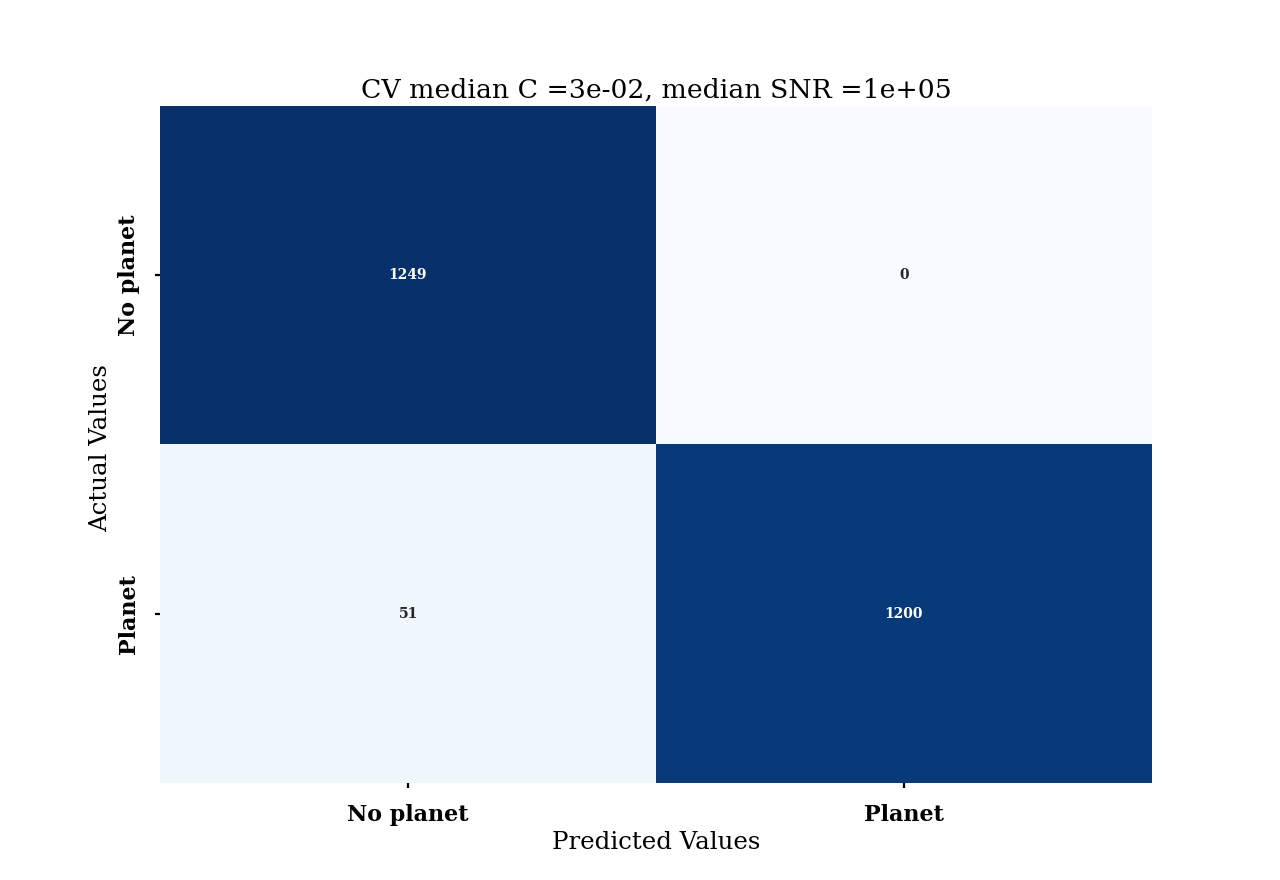
\includegraphics[scale=0.3]{images/Chapter3/confusion_RF_CV_1e-02_cmax_1e-01_dsnrmin_1e+04_dsnrmax_1e+06.png}
    \caption{Caption}
    \label{fig:RF1e-1-1e-2}
\end{subfigure}
\hfill
\begin{subfigure}{0.4\textwidth}
    \centering
    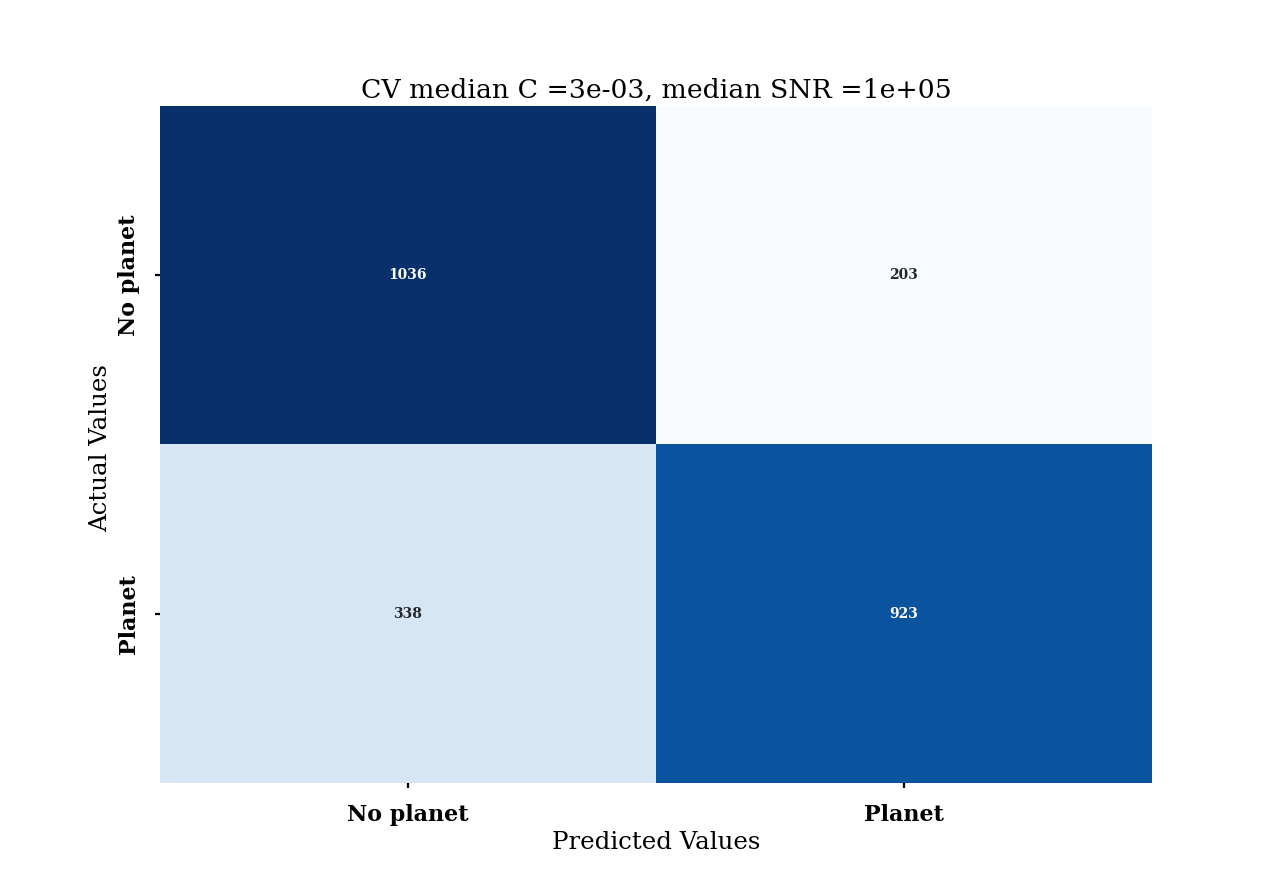
\includegraphics[scale=0.3]{images/Chapter3/confusion_RF_CV_1e-03_cmax_1e-02_dsnrmin_1e+04_dsnrmax_1e+06.png}
    \caption{Caption}
    \label{fig:RF1e-3_1e-2}
\end{subfigure}
\caption{RF results}
\end{figure}
\begin{figure}[!hb]
\begin{subfigure}{0.4\textwidth}
    \centering
    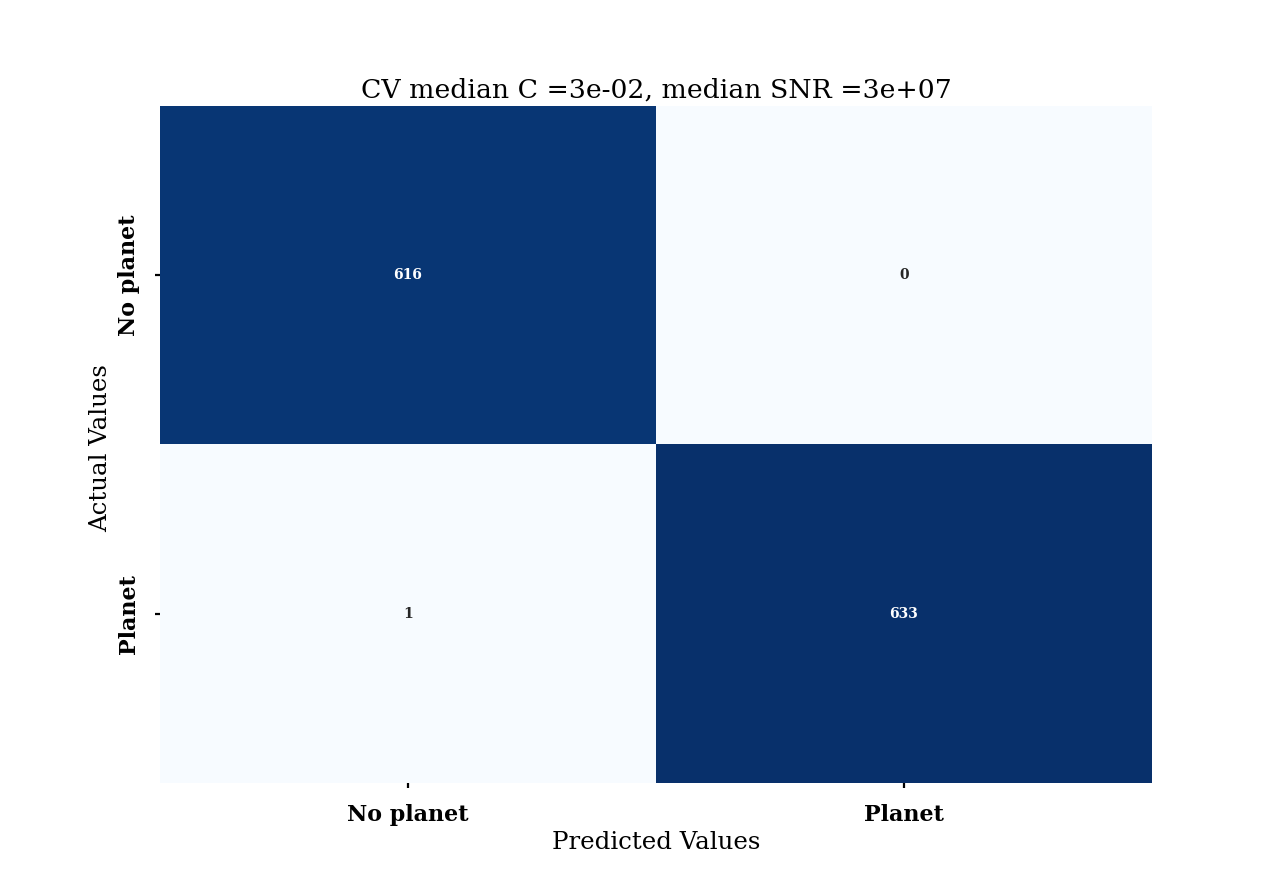
\includegraphics[scale=0.25]{images/Chapter3/confusion_transfer_sdae_CV_cmin_1e-02_cmax_1e-01_dsnrmin_1e+07_dsnrmax_1e+08.png}
    \caption{Caption}
    \label{fig:ae1e-2_1e-1}
\end{subfigure}
\hfill
\begin{subfigure}{0.4\textwidth}
    \centering
    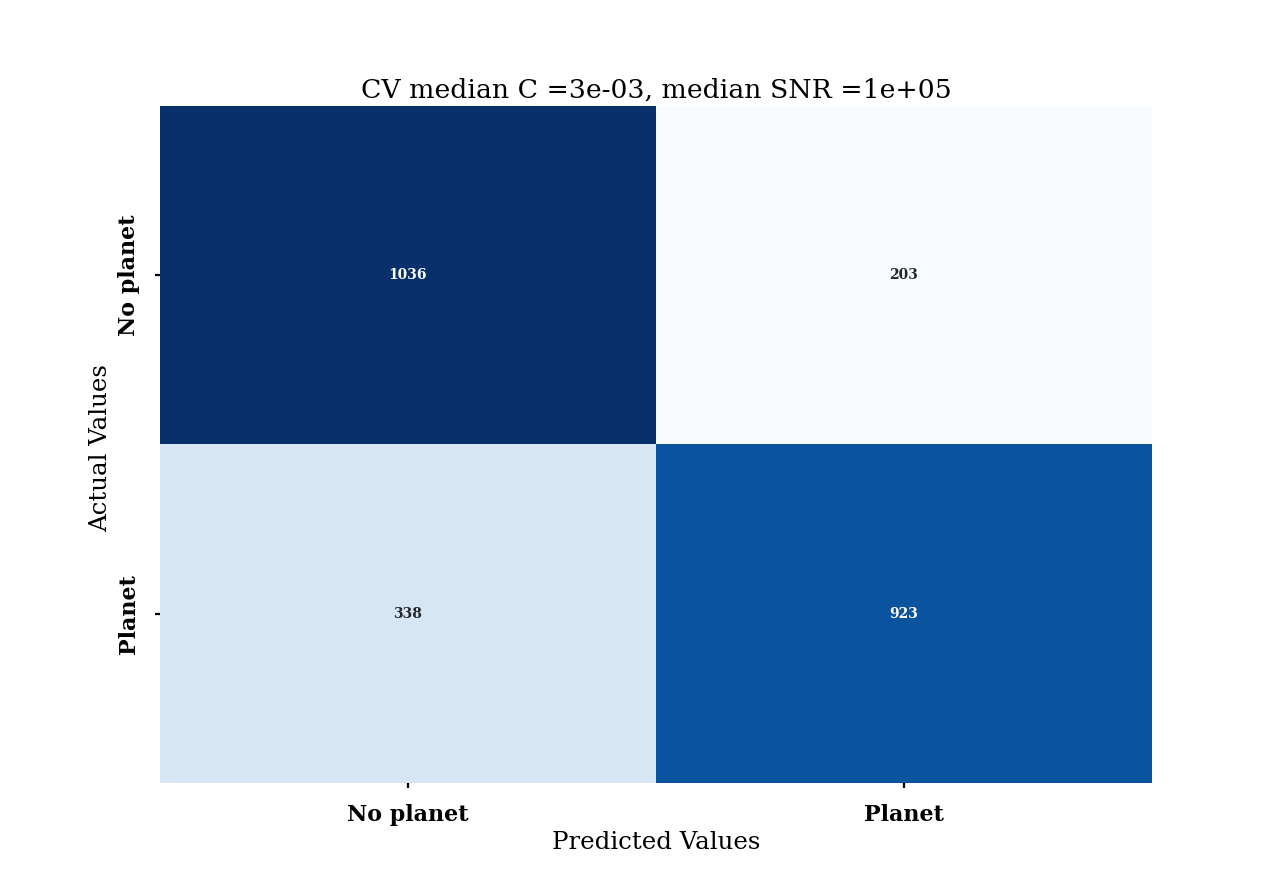
\includegraphics[scale=0.3]{images/Chapter3/confusion_RF_CV_1e-03_cmax_1e-02_dsnrmin_1e+04_dsnrmax_1e+06.png}
    \caption{Caption}
    \label{fig:ae1e-3_1e-2}
\end{subfigure}
\caption{AE results}
\end{figure}
When comparing the low contrast results its very interesting to look at \Cref{fig:ccf_cm} and \Cref{fig:RF1e-3_1e-2} and \Cref{fig:ae1e-3_1e-2} which are tested around the same contrasts.
The number of false positives is $0$ for the cross correlation and is $\approx 200$ for the ML aglorithms.
Note that this number is $\approx 10$ for a lower contrast on the left.
The $TPR\approx0.75$ for the ML algorithms but for the cross correlation based algorithm $\rm{TPR}=1$.
This is an interesting feature that when the contrast increases even in the low contrast cases the $\rm{TPR}$ plummets by a $\approx1/3$ and the number of false positives increases from $0$ to $200$.
Note that while the $\rm{TPR}$ remains high enough for the algorithm to be considered successful for mean $C\approx10^{-3}$, the number of false positives would deem the algorithm unsuitable for scientific usages.
At this stage, we can  say that ML algorithms have not achieved the necessary false positive requirement for scientific analysis.
However, in order to understand at what contrast the ML algorithms no longer learn new features we will also present the high contrast results.
\subsection{high contrast results}
We define a high contrast spectrum as that where $C<10^{-3}$.
We have already such a case of confusio matrix being produced for \Cref{fig:high contrast-ccf cm} where we see that $1$ false positive is identified for $10^{4}$ spectra  and the $\rm{TPR}\approx 0.7$.
We will now train and test this data with ML algorithms and these results are depicted in \Cref{fig:highcont_rf}
\begin{figure}
\begin{subfigure}{0.4\textwidth}
        \centering
        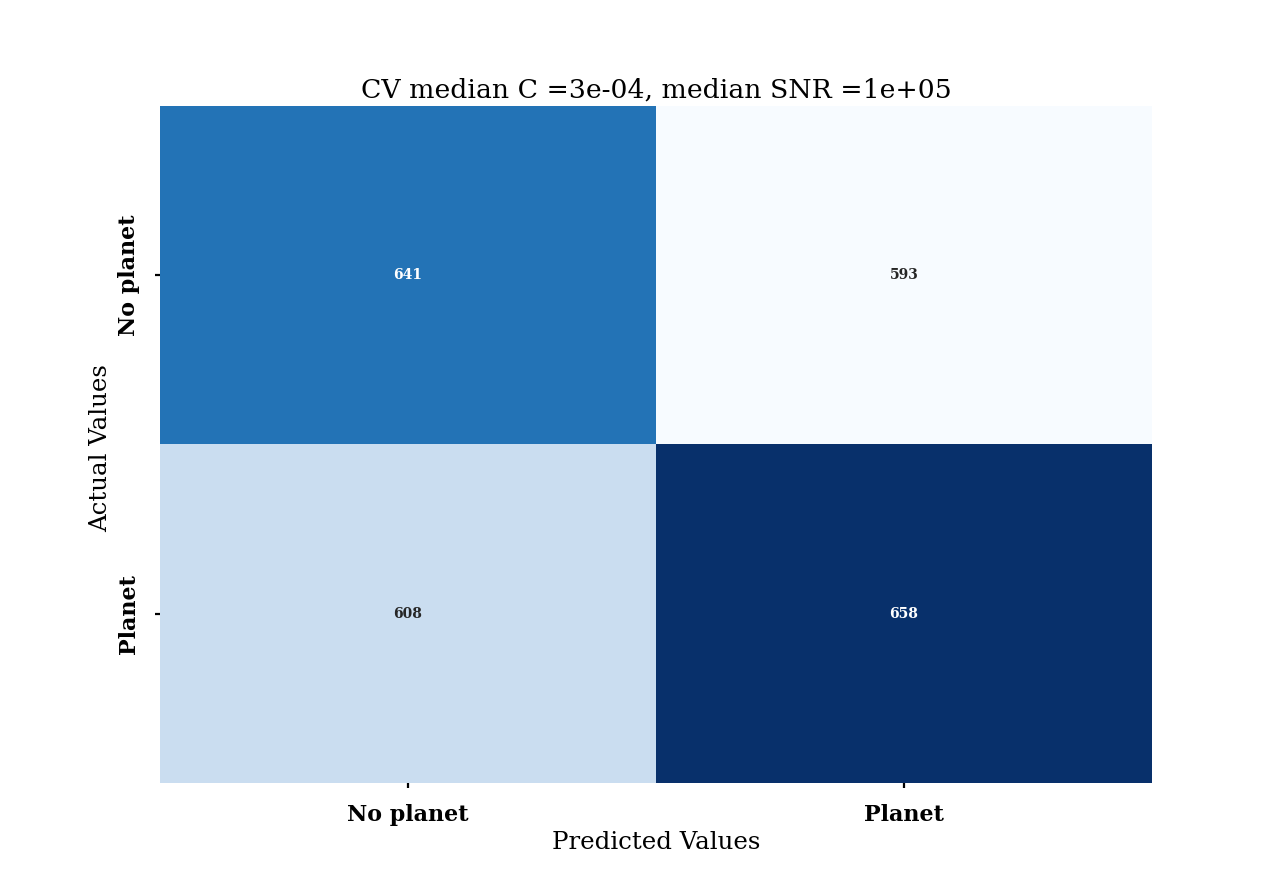
\includegraphics[scale=0.3]{images/Chapter3/confusion_RF_CV_1e-04_cmax_1e-03_dsnrmin_1e+04_dsnrmax_1e+06.png}
        \caption{Caption}
        \label{fig:highcont_rf}
\end{subfigure}
\hfill
\begin{subfigure}{0.4\textwidth}
        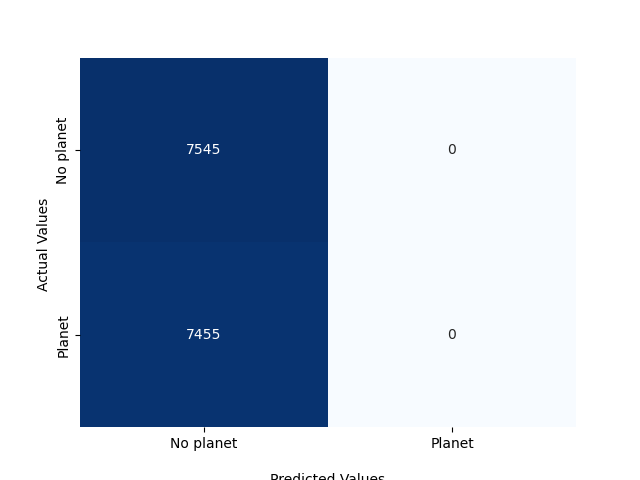
\includegraphics[scale=0.4]{images/Chapter3/confusion_mlp_1e-5_keras_train.png}
        \caption{Caption}
        \label{fig:highcont_mlp}
\end{subfigure}
\vfill
\begin{subfigure}{0.5\textwidth}
        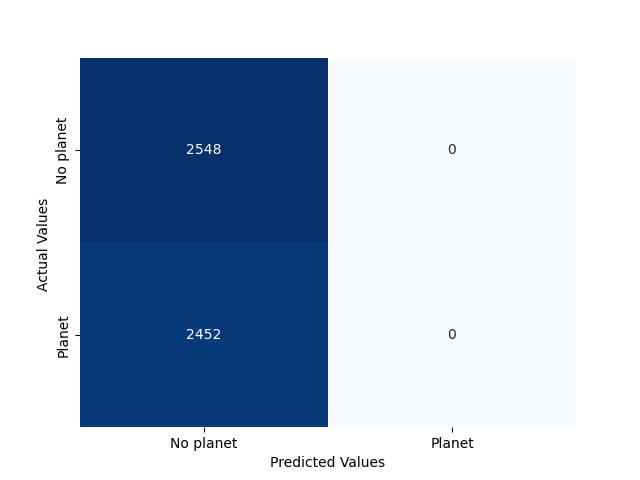
\includegraphics[scale=0.4]{images/Chapter3/confusion_ae_CV_lowcont_1e-5.png}
        \caption{Caption}
        \label{fig:highcont_ae}
\end{subfigure}
\label{figs:highcont}
\end{figure}
\textcolor{blue}{[TODO: 1. Training CM for both low and high contrast for all the algorithms
2. Make sure the CM are in the same SNR 
3. Have CM from two different ranges of SNR so its clear that its only contrast and not SNR which is the problem]}
\section{Discussion}
In this chapter, we have explored the use of three different ML algorithms in testing the detection hypothesis.
We were unable to progress beyond  testing the algorithms themselves to subsequently test the hypotheses themselves.
In this discussion section we will discuss what are the reasons for the poor results from ML algorithms.
\subsection{Random forest feature importances}
From the confusion matrices \Cref{fig:ae1e-2_1e-1} and \Cref{fig:RF1e-1-1e-2} it is clear that the training on very low contrasts where the planet is about $10$th as bright as the host star allows the ML algorithms to train effectively and produce the necessary confusion matrices as desired by our problem statement.
From these confusion matrices, it appears that as we increase the contrast the ability to classify drops off quite rapidly.
If this is indeed the case, what features does the ML algorithm learn in the lowest contrast that seem to disappear in the higher contrasts.
In order to answer this question we performed a very specific experiment by generating spectra for an exoplanet with exactly the same $\rm{T_{eff}}$ and $\rm{\log(g)}$ and train the random forest for different contrasts.
Note that even this case we get the exact same confusion matrices.
\begin{figure}
    \centering
    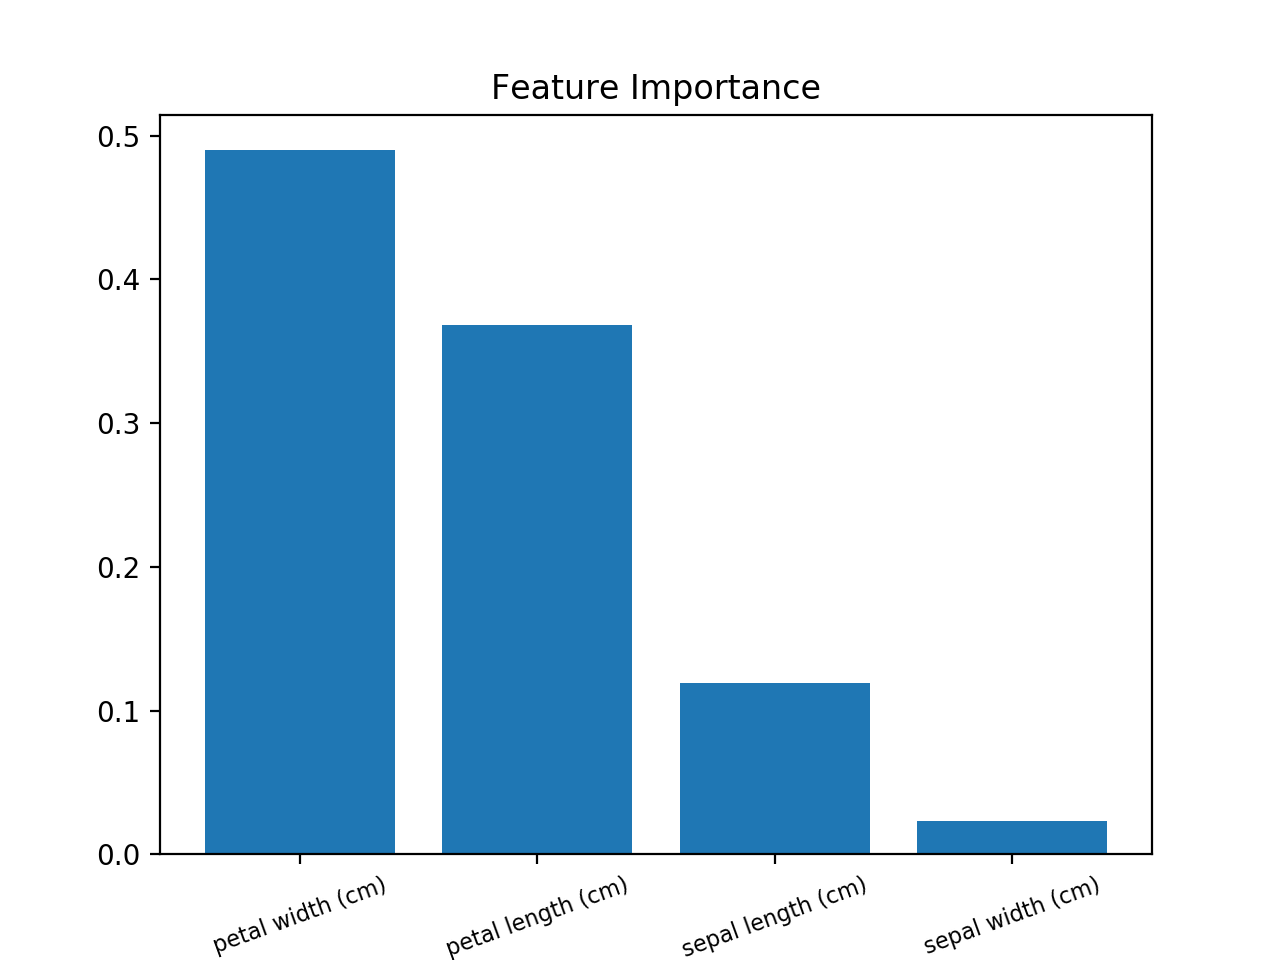
\includegraphics[scale=0.5]{images/Chapter3/feature_importances_Randomforest.png}
    \caption{Caption}
    \label{fig:RF-C-importances}
\end{figure}
Thus we produce \Cref{fig:RF-C-importances} using the same $\rm{SNR}$ and different values $C$.
The feature importances are plotted as function of $\lambda$ and should therefore track the importance of the wavelength bins.
In this figure, the uppermost dark panel indicates the template that was used to generate spectra to train with different contrasts.
The lower panels indicate the featrue importances produced by different random forest models.
The goal of our training is to generate feature importances that are a mirror image of the first panel in this image.
The first panel in this image represents the spectral features which are unique to an exoplanet that are not shared by either the noise or the stellar spectrum. 
This means that the features that the ML algorithms need to learn are the features uniquely present in the exoplanet spectrum. 
By training the ML algorithms with different types of spectra, we attempted to produce a plethora of features that would allow an ML algorithm to generalize. 
However, even when we restrict this problem to exactly one type of exoplanet we see that the features learnt with the changing contrasts are highly limited by the contrast.

One of the first noteworthy things about \Cref{fig:RF-C-importances} is the low values of the feature importances when compared to more `classical' feature importances such as \Cref{fig:RF sample FI}. 
While there is a relative gradient at the lowest contrast, the mean value is quite low.
This of course is a function of having a large number of absorption features which means that when no one feature is more important than the others we will have the importances distributed over many wavelengths. 
Our view on this plot is that while there does seem to be some amount of learning of the relative importances,the extremely low value of each importance actually seems to indicate that the model is unable to train robustly and learn all the features.
The second noteworthy point on this graph is the virtual disappearance of importances as the contrast increases and $C$ value decreases.
There seems to be some type of overfitting for the noise we can see a slight curving of the importances with the increasing wavelength.
When we look at the same feature importances for a low contrast and changing $\rm{SNR}$ we can see the same kind of behaviour in \Cref{fig: RF-SNR-featureimportances}.
We see that for the highest $\rm{SNR}$ the feature importances follow the same pattern as in \Cref{fig:RF-C-importances} and then for the same low contrast spectrum we see the feature importances disappearing as we decrease $\rm{SNR}$.
\begin{figure}
    \centering
    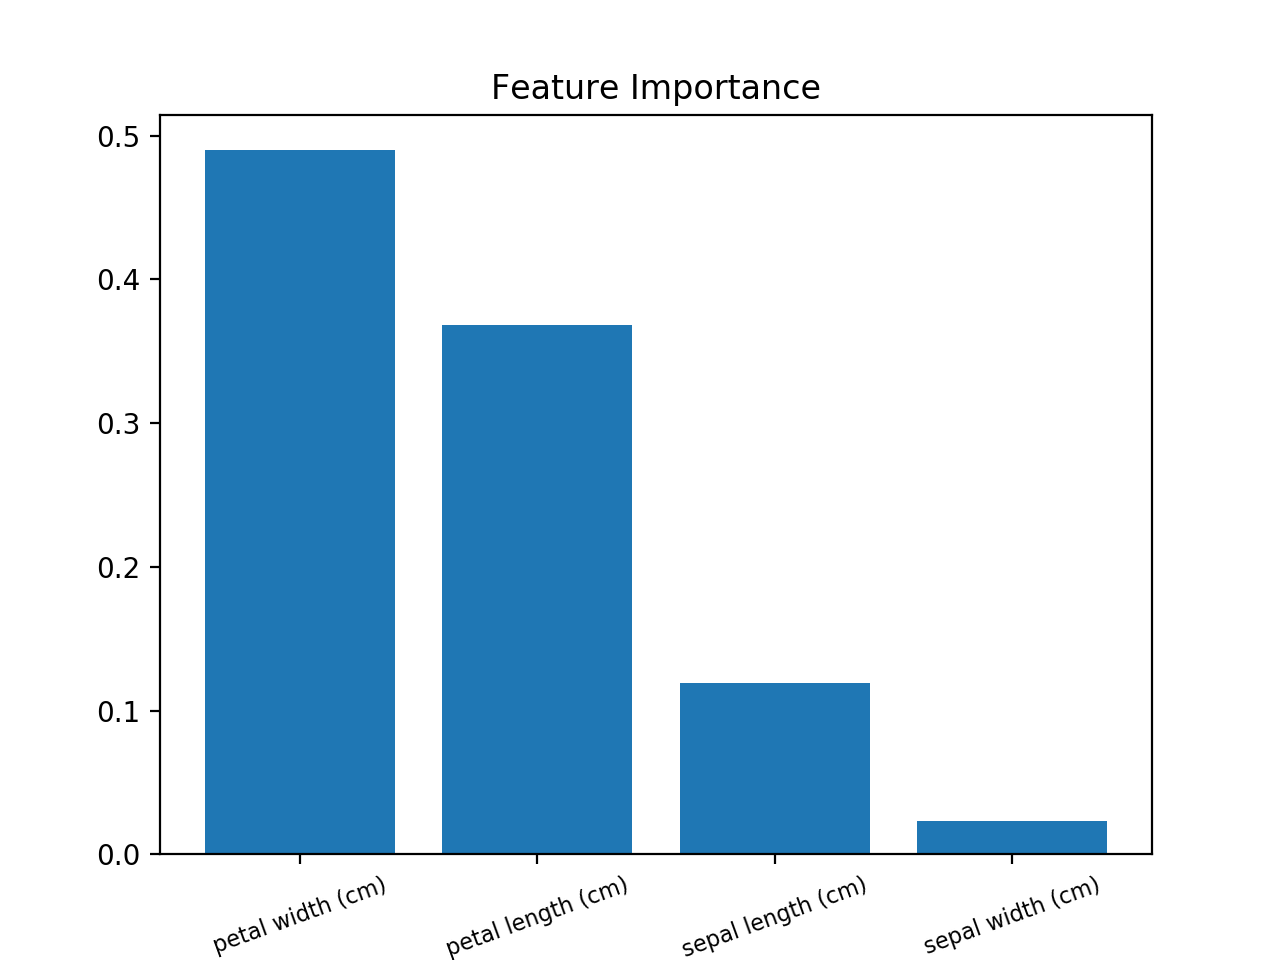
\includegraphics[scale=0.5]{images/Chapter3/feature_importances_Randomforest.png}
    \caption{\textcolor{blue}{Use the correct plot here}}
    \label{fig: RF-SNR-featureimportances}
\end{figure}
This behaviour attests to the most important inference of this part of my thesis,
In order for ML algorithms to be able to train and generalize on spectra from direct images the data needs to be both low contrast and high $\rm{SNR}$ as described in \Cref{chap:III.3}.
In the next subsection we will discuss why this form of problem statement is not very appropriate for ML algorithms.

\subsection{On the unsuitability of ML algorithms to test the detection and characterization hypotheses}
At the beginning of this part in \Cref{chap: III.1}, we stated that ML algorithms had the ability to process multiple datasets rapidly and with high precision. 
We also stated the ability of ML algorithms to draw inferences from diverse data sources.
In that sense we have developed our ML based algorithms to train on spectral data from multiple spectral channels.
We have identified the `best' quality data by defining a $\rm{SNR}$ which is a pure signal metric to define a spectrum.
We have also used $C$ as a parameter to inject astrophysics into the problem.
But these have served only as scaffolding to the fundamental question, which is whether given diverse spectral features in a high quality astrophysical spectrum can an ML algorithm train and generalize to detect exoplanets and further to characterize them.
To this effect we trained an ensemble algorithm and two deep learning algorithms.
We found that the best spectra to train were indeed the ones with lowest contrast and highest $\rm{SNR}$.
We also learnt that the features that for example a random forest based algorithm learns is a mild version of the spectral features shows that ML algorithms are indeed capable of learning some features.
However, what is also clear is that ML algorithms are not able to diversify these features to pick up higher contrast or lower $\rm{SNR}$ exoplanets in spectra.

To verify that the features are not transferrable, we saved the weights of the deep learning algorithms and used them as the starting weights to train higher contrast companions. 
We found that the confusion matrices are exactly the same. 
When we tried to use the same weights tuned to detect lower contrast exoplanets we found that the neural network never detects the exoplanet. 
This means that the features learnt on low contrast or high $\rm{SNR}$ are not general enough to be used to detect exoplanets.
This is the fundamental reason why we cannot compose a detection matrix using ML algorithms.
Consequently, we cannot test the detection hypothesis using ML algorithms.

The characterization hypothesis, relies on the ability of an algorithm to primarily detect the spectrum. 
We saw with the cross correlation based algorithm that when an exoplanet is detectable in the spectrum, it can be characterized with a consistent error bar which in turn can be reduced by perfectly dividing out the stellar contamination.
However, ML algorithms have proven to be incompetent in learning features to even test the detection hypothesis and therefore it does not behove to test the characterization hypothesis which relies on the very same features.
Note that this thesis has stopped short of composing the characterization matrix for those exoplanet spectra that can be detected due to the lack of time.

\chapter{Use of machine learning algorithms with map based data}
This is section 3 and4 of the paper
\section{Computer vision and its capabilities}
\section{Development of C3PO}
\section{Development of C-LANDO}
\section{Interpreting the output of ML algorithms}

\chapter{Training and testing of the ML algorithms with simulated data}
This is section 5 of the paper to define how we plan to use the algorithms together


\chapter{Discussion and salient features of map based detection algorithms}
Section 6 and 7 of the paper but also discuss why this stuff is good for benchmarking datasets.
